\documentclass{article}
\usepackage{graphicx}
\usepackage{subcaption}
\usepackage{geometry}
\usepackage{hyperref}
\usepackage{grffile} % To handle dots and special characters in filenames

\geometry{
    a4paper,
    margin=0.8in
}

\hypersetup{
    colorlinks=true,
    linkcolor=blue,
    filecolor=magenta,      
    urlcolor=cyan,
}

\title{Byzantine Robustness Comparison:\\CNN vs. SNN (Simplest Sweeps)}
\author{ByzFL SNN Benchmark}
\date{\today}

\begin{document}

\maketitle

\tableofcontents
\newpage

\section{Introduction}
This document presents side-by-side comparison grids of Byzantine robustness results for CNN and SNN architectures under the simplest sweep configurations. The configurations compared are:
\begin{enumerate}
    \item \textbf{CNN}: Convolutional Neural Network on MNIST (`cnn\_simplest\_plots`)
    \item \textbf{SNN}: Spiking Neural Network on MNIST (`snn\_simplest\_plots`)
\end{enumerate}

Each grid illustrates the test accuracy under varying numbers of Byzantine clients ($f \in [0, 2, 4, 5]$) and data heterogeneity levels ($\gamma \in [0.0, 0.33, 0.66, 1.0]$) with $N = 10$ honest clients.

\newpage

\section{Worst-Case Performance (Across All Attacks)}
\label{sec:worst_case}
This section compares the test accuracy under the worst-case attack scenario (minimizing the maximum damage over all attacks) for both the dynamically selected best aggregator and each of the fixed aggregators.

\subsection{Best Aggregator Choice}
\begin{figure}[htbp]
    \centering
    \begin{subfigure}[b]{0.49\textwidth}
        \centering
        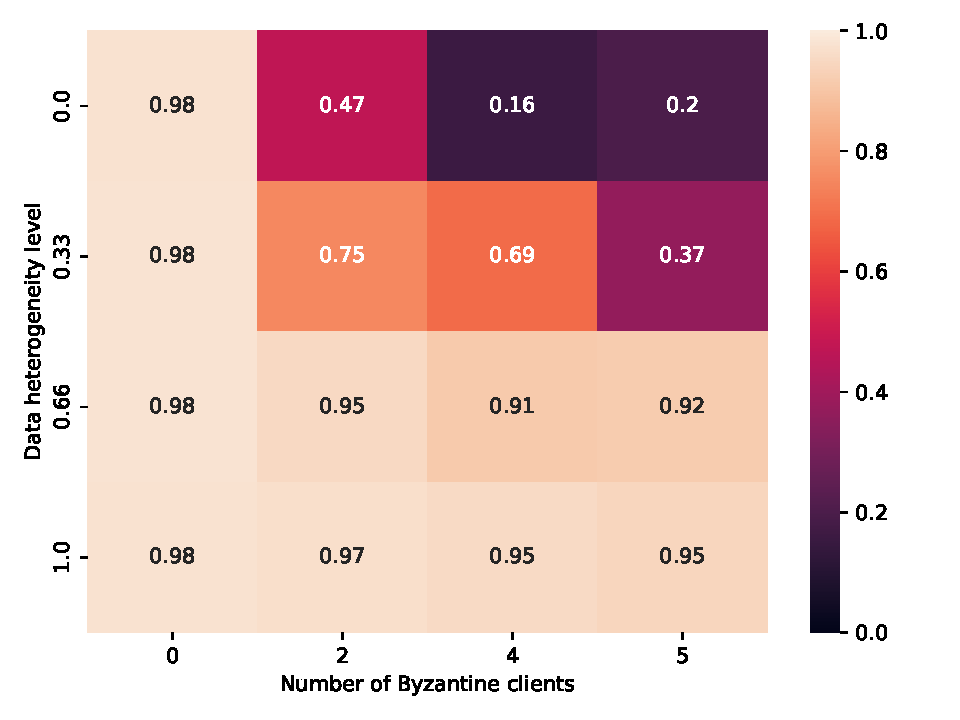
\includegraphics[width=\textwidth]{cnn_simplest_plots/best_test_mnist_cnn_mnist_gamma_similarity_niid_NNM_ARC_nb_honest_clients_10_tolerated_f_equal_real.pdf}
        \caption{CNN (Best Aggregator Choice)}
        \label{fig:best_choice_cnn}
    \end{subfigure}
    \hfill
    \begin{subfigure}[b]{0.49\textwidth}
        \centering
        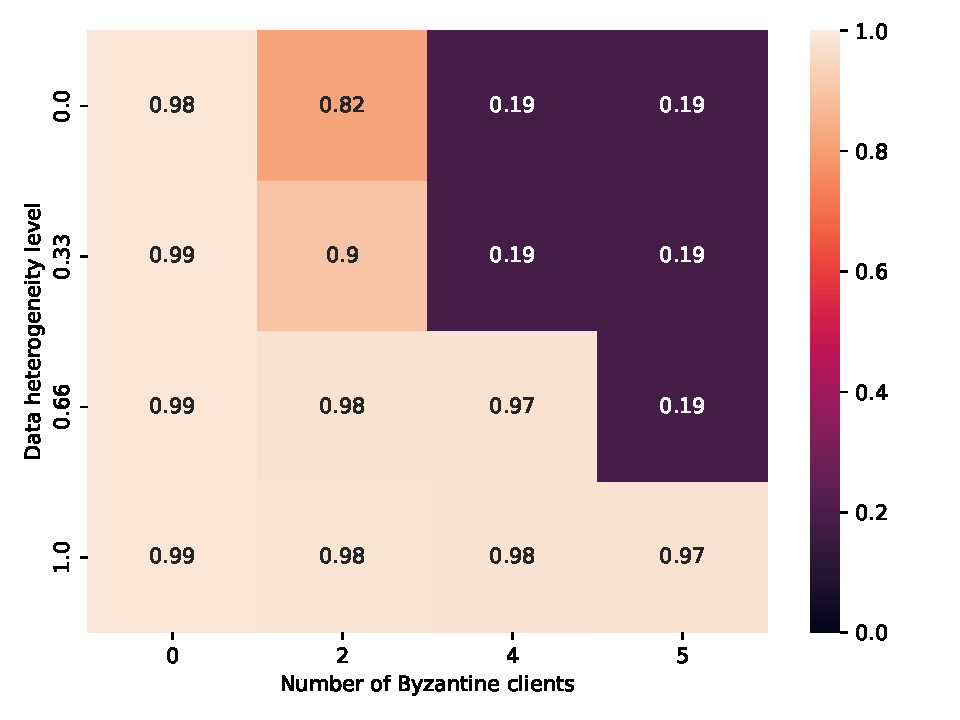
\includegraphics[width=\textwidth]{snn_simplest_plots/best_test_mnist_cnn_mnist_snn_gamma_similarity_niid_NNM_ARC_nb_honest_clients_10_tolerated_f_equal_real.pdf}
        \caption{SNN (Best Aggregator Choice)}
        \label{fig:best_choice_snn}
    \end{subfigure}
    \caption{Worst-case test accuracy comparison using the best overall aggregator selection.}
    \label{fig:best_overall}
\end{figure}

\clearpage

\subsection{Centered Clipping}
\begin{figure}[htbp]
    \centering
    \begin{subfigure}[b]{0.49\textwidth}
        \centering
        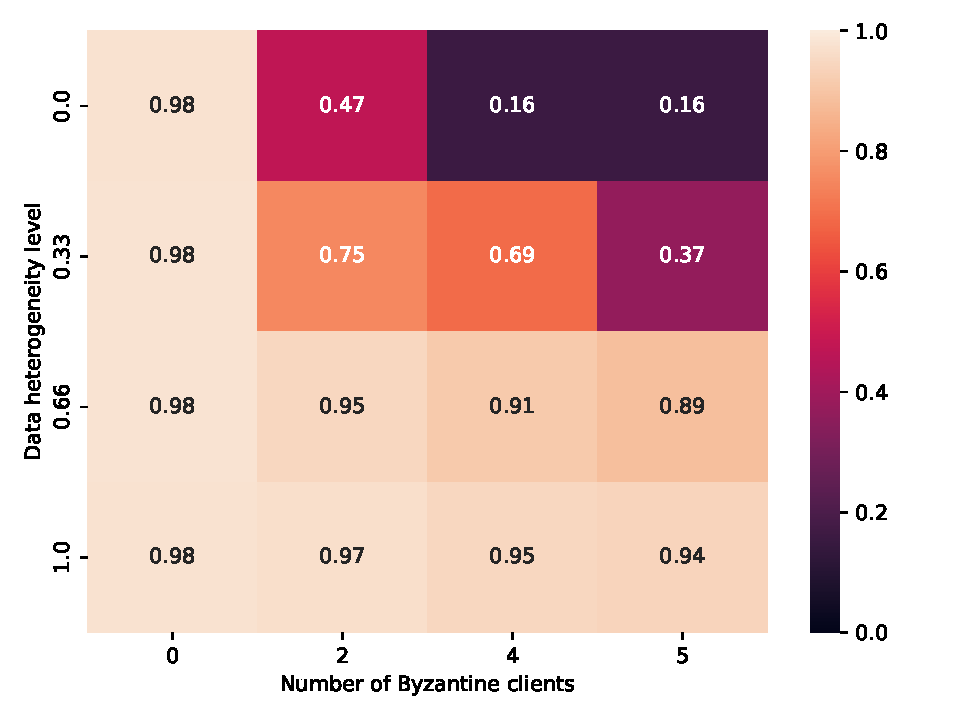
\includegraphics[width=\textwidth]{cnn_simplest_plots/test_mnist_cnn_mnist_gamma_similarity_niid_NNM_ARC_CenteredClipping_nb_honest_clients_10_tolerated_f_equal_real.pdf}
        \caption{CNN (Centered Clipping)}
        \label{fig:cc_cnn}
    \end{subfigure}
    \hfill
    \begin{subfigure}[b]{0.49\textwidth}
        \centering
        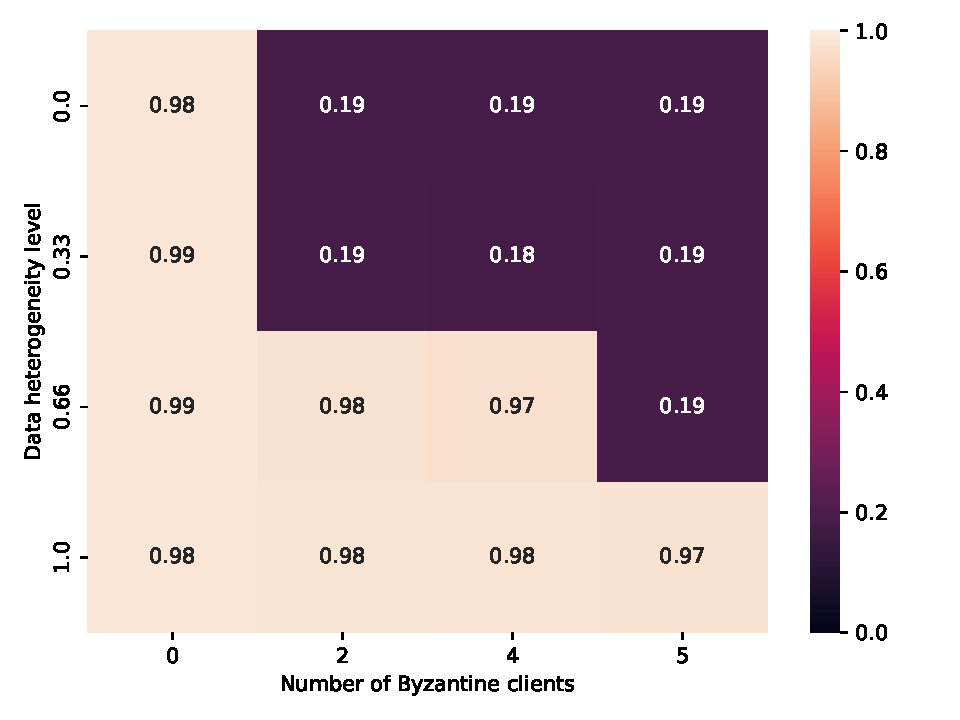
\includegraphics[width=\textwidth]{snn_simplest_plots/test_mnist_cnn_mnist_snn_gamma_similarity_niid_NNM_ARC_CenteredClipping_nb_honest_clients_10_tolerated_f_equal_real.pdf}
        \caption{SNN (Centered Clipping)}
        \label{fig:cc_snn}
    \end{subfigure}
    \caption{Worst-case test accuracy comparison using Centered Clipping.}
    \label{fig:cc_comparison}
\end{figure}

\clearpage

\subsection{Geometric Median}
\begin{figure}[htbp]
    \centering
    \begin{subfigure}[b]{0.49\textwidth}
        \centering
        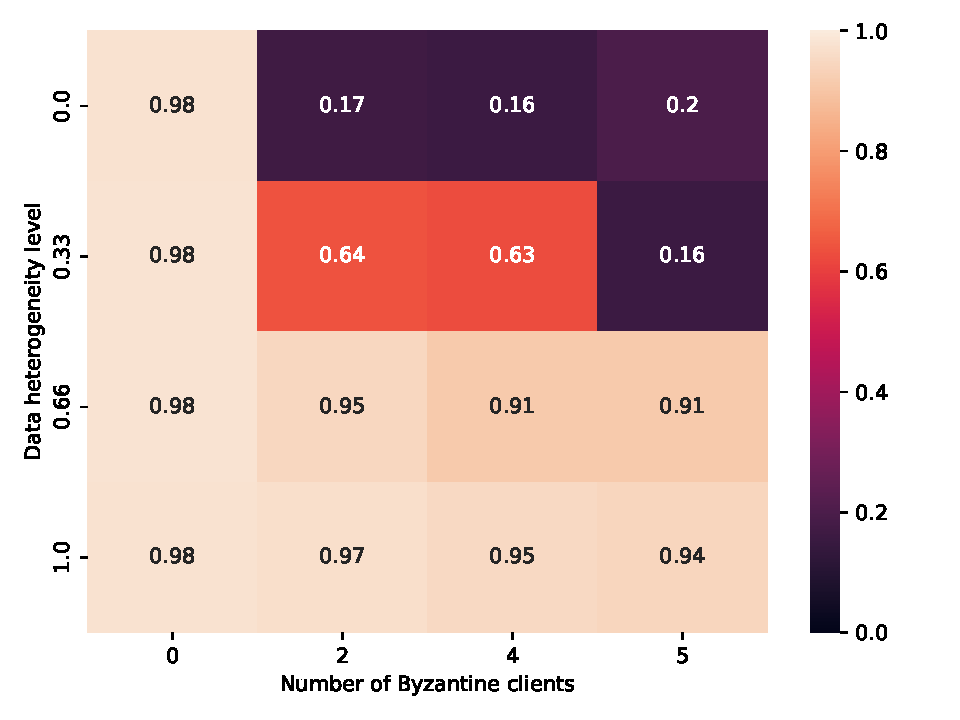
\includegraphics[width=\textwidth]{cnn_simplest_plots/test_mnist_cnn_mnist_gamma_similarity_niid_NNM_ARC_GeometricMedian_nb_honest_clients_10_tolerated_f_equal_real.pdf}
        \caption{CNN (Geometric Median)}
        \label{fig:gm_cnn}
    \end{subfigure}
    \hfill
    \begin{subfigure}[b]{0.49\textwidth}
        \centering
        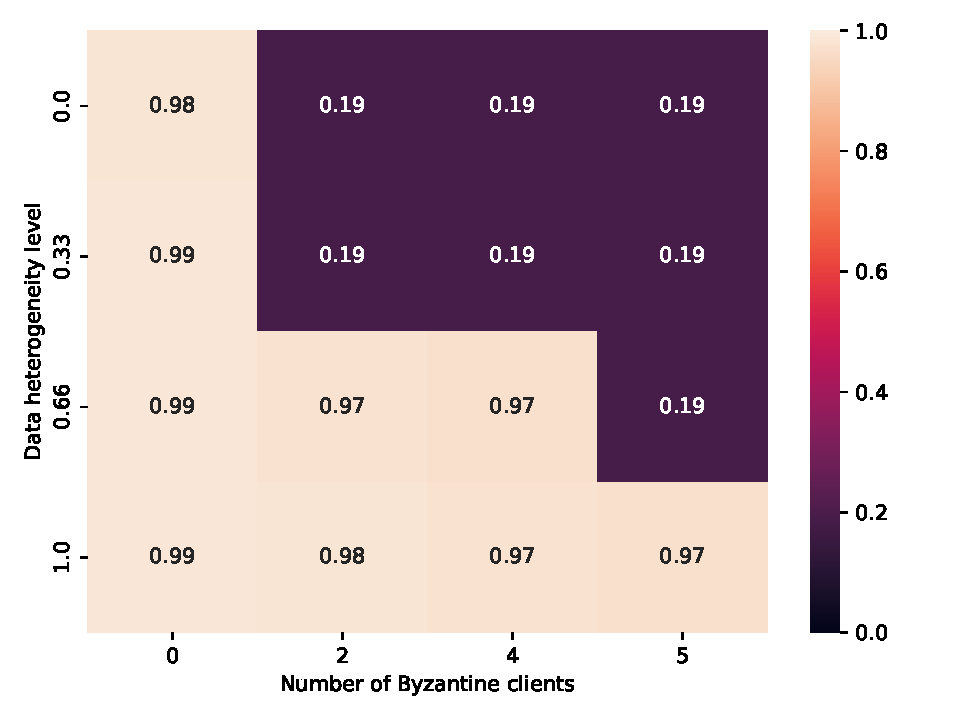
\includegraphics[width=\textwidth]{snn_simplest_plots/test_mnist_cnn_mnist_snn_gamma_similarity_niid_NNM_ARC_GeometricMedian_nb_honest_clients_10_tolerated_f_equal_real.pdf}
        \caption{SNN (Geometric Median)}
        \label{fig:gm_snn}
    \end{subfigure}
    \caption{Worst-case test accuracy comparison using Geometric Median.}
    \label{fig:gm_comparison}
\end{figure}

\clearpage

\subsection{Multi-Krum}
\begin{figure}[htbp]
    \centering
    \begin{subfigure}[b]{0.49\textwidth}
        \centering
        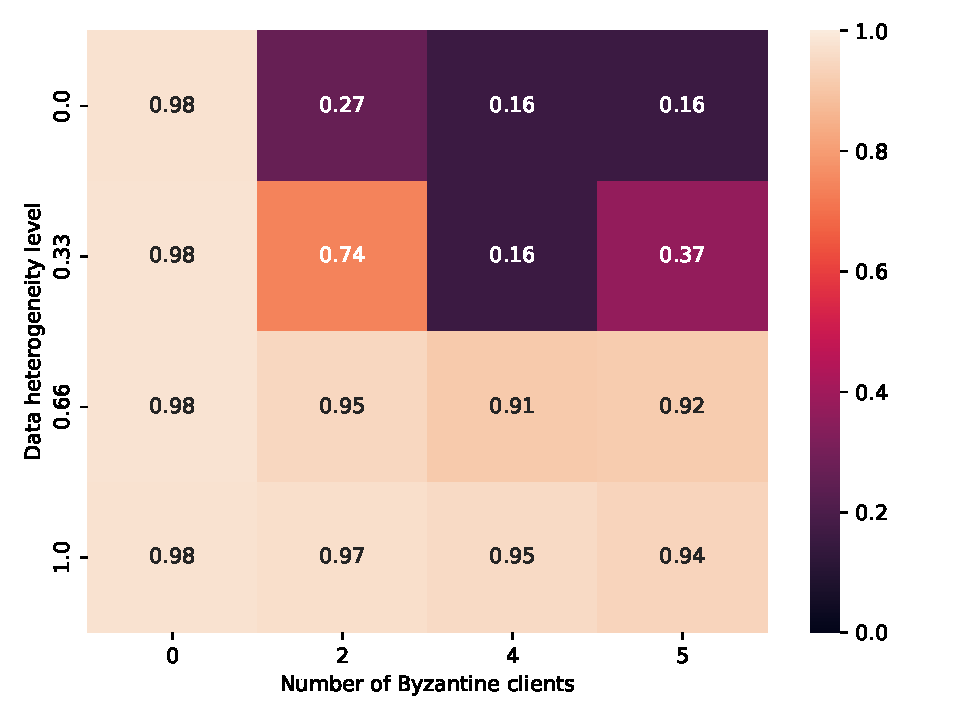
\includegraphics[width=\textwidth]{cnn_simplest_plots/test_mnist_cnn_mnist_gamma_similarity_niid_NNM_ARC_MultiKrum_nb_honest_clients_10_tolerated_f_equal_real.pdf}
        \caption{CNN (Multi-Krum)}
        \label{fig:mk_cnn}
    \end{subfigure}
    \hfill
    \begin{subfigure}[b]{0.49\textwidth}
        \centering
        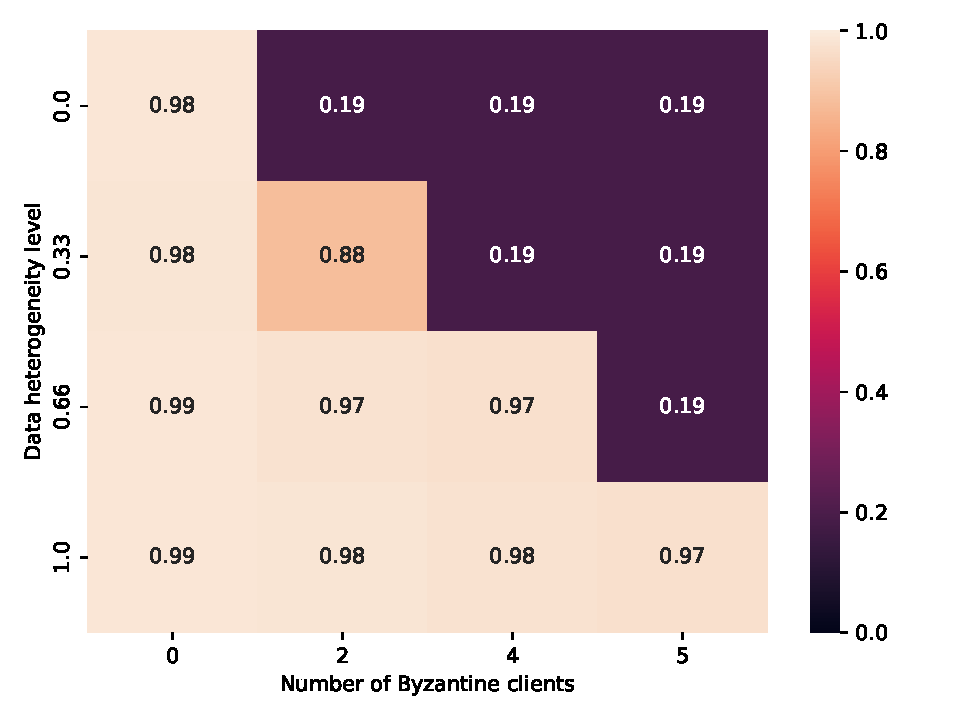
\includegraphics[width=\textwidth]{snn_simplest_plots/test_mnist_cnn_mnist_snn_gamma_similarity_niid_NNM_ARC_MultiKrum_nb_honest_clients_10_tolerated_f_equal_real.pdf}
        \caption{SNN (Multi-Krum)}
        \label{fig:mk_snn}
    \end{subfigure}
    \caption{Worst-case test accuracy comparison using Multi-Krum.}
    \label{fig:mk_comparison}
\end{figure}

\clearpage

\subsection{Trimmed Mean}
\begin{figure}[htbp]
    \centering
    \begin{subfigure}[b]{0.49\textwidth}
        \centering
        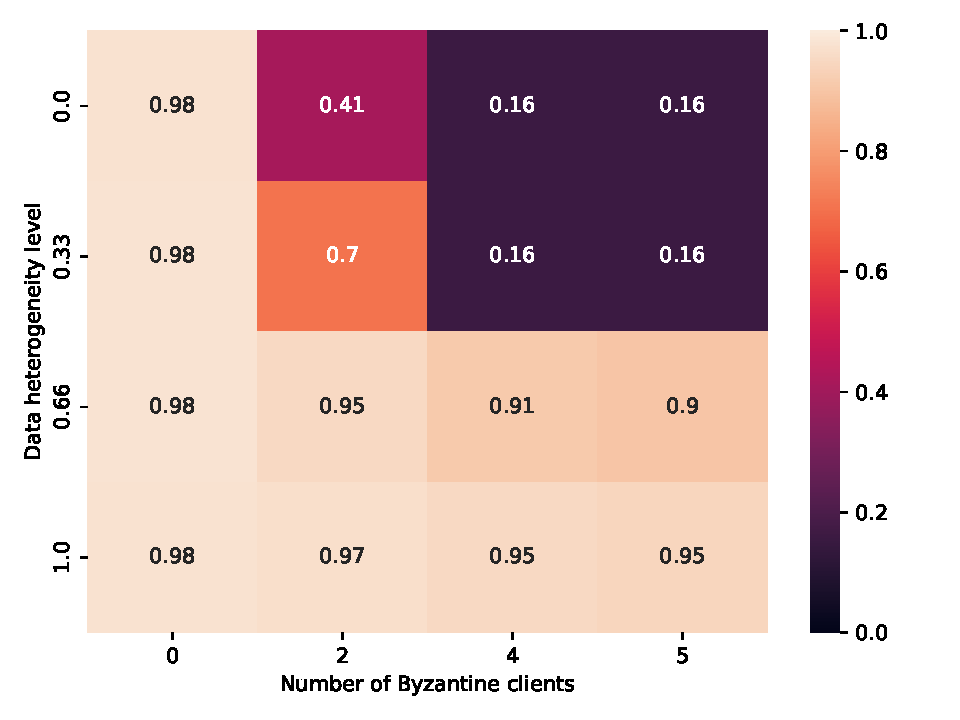
\includegraphics[width=\textwidth]{cnn_simplest_plots/test_mnist_cnn_mnist_gamma_similarity_niid_NNM_ARC_TrMean_nb_honest_clients_10_tolerated_f_equal_real.pdf}
        \caption{CNN (Trimmed Mean)}
        \label{fig:tm_cnn}
    \end{subfigure}
    \hfill
    \begin{subfigure}[b]{0.49\textwidth}
        \centering
        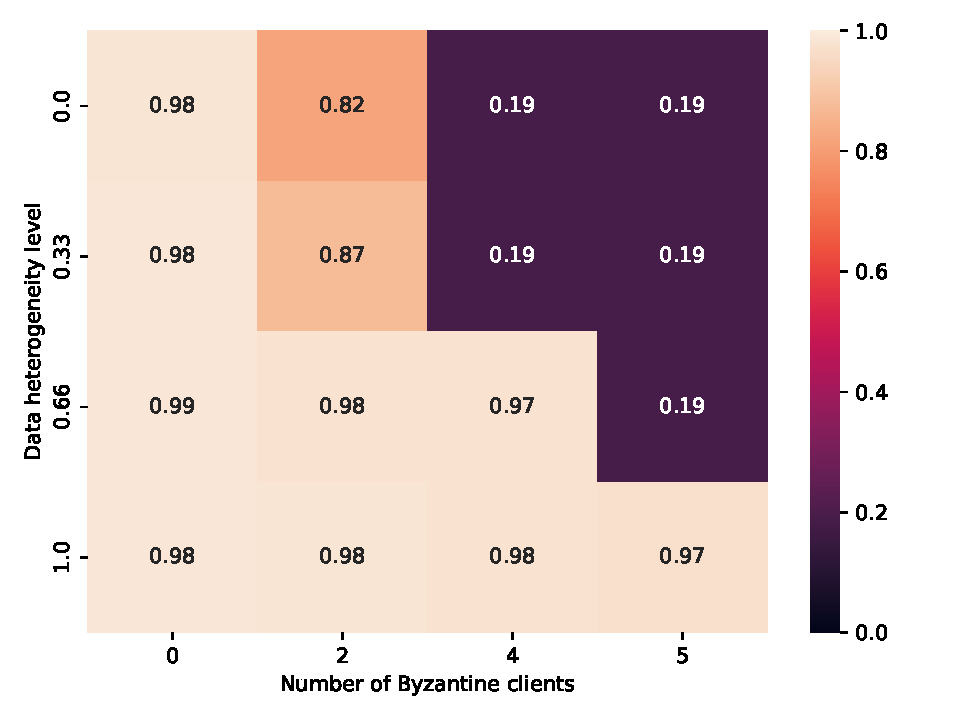
\includegraphics[width=\textwidth]{snn_simplest_plots/test_mnist_cnn_mnist_snn_gamma_similarity_niid_NNM_ARC_TrMean_nb_honest_clients_10_tolerated_f_equal_real.pdf}
        \caption{SNN (Trimmed Mean)}
        \label{fig:tm_snn}
    \end{subfigure}
    \caption{Worst-case test accuracy comparison using Trimmed Mean.}
    \label{fig:tm_comparison}
\end{figure}

\clearpage

\section{Fixed Attack: Optimal A Little Is Enough (ALIE)}
\label{sec:alie_attack}
This section compares performance under the Optimal ALIE Byzantine attack, showing both the dynamically selected best aggregator and each of the fixed aggregators.

\subsection{Best Aggregator Choice}
\begin{figure}[htbp]
    \centering
    \begin{subfigure}[b]{0.49\textwidth}
        \centering
        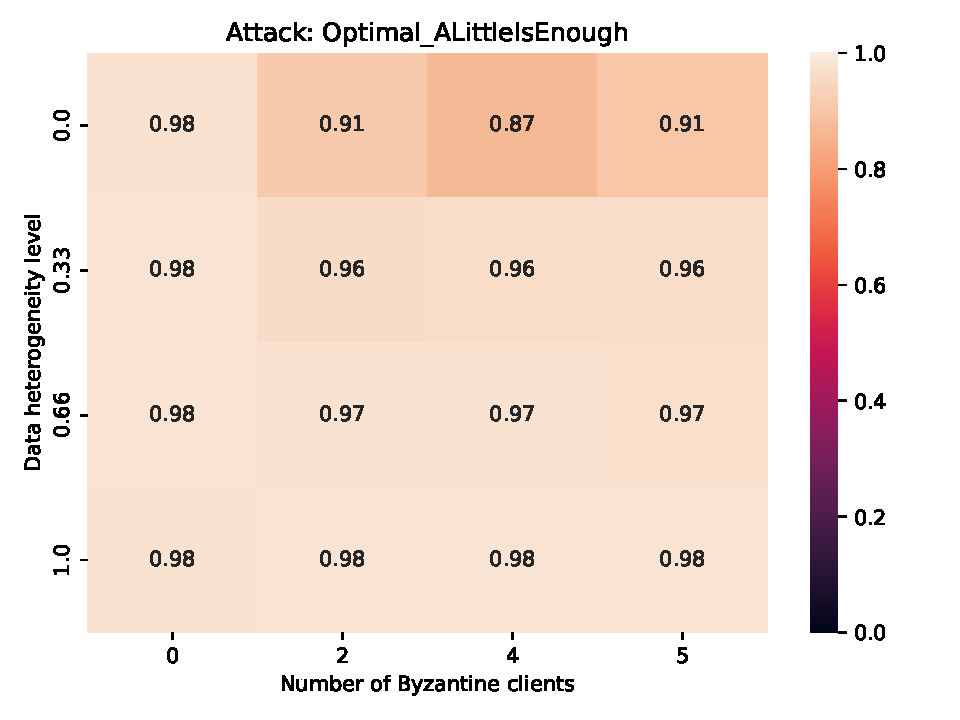
\includegraphics[width=\textwidth]{cnn_simplest_plots/best_test_Optimal_ALittleIsEnough_mnist_cnn_mnist_gamma_similarity_niid_NNM_ARC_nb_honest_clients_10_tolerated_f_equal_real.pdf}
        \caption{CNN (Best Aggregator Choice)}
        \label{fig:alie_best_cnn}
    \end{subfigure}
    \hfill
    \begin{subfigure}[b]{0.49\textwidth}
        \centering
        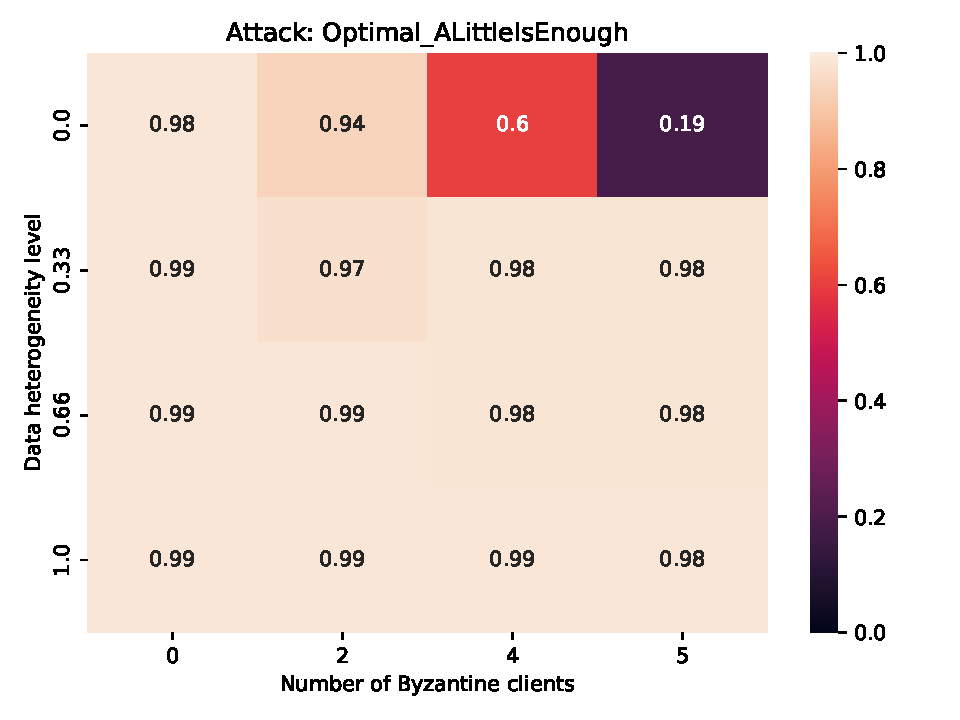
\includegraphics[width=\textwidth]{snn_simplest_plots/best_test_Optimal_ALittleIsEnough_mnist_cnn_mnist_snn_gamma_similarity_niid_NNM_ARC_nb_honest_clients_10_tolerated_f_equal_real.pdf}
        \caption{SNN (Best Aggregator Choice)}
        \label{fig:alie_best_snn}
    \end{subfigure}
    \caption{Accuracy comparison under Optimal ALIE attack using the best aggregator selection.}
    \label{fig:alie_best_overall}
\end{figure}

\clearpage

\subsection{Centered Clipping}
\begin{figure}[htbp]
    \centering
    \begin{subfigure}[b]{0.49\textwidth}
        \centering
        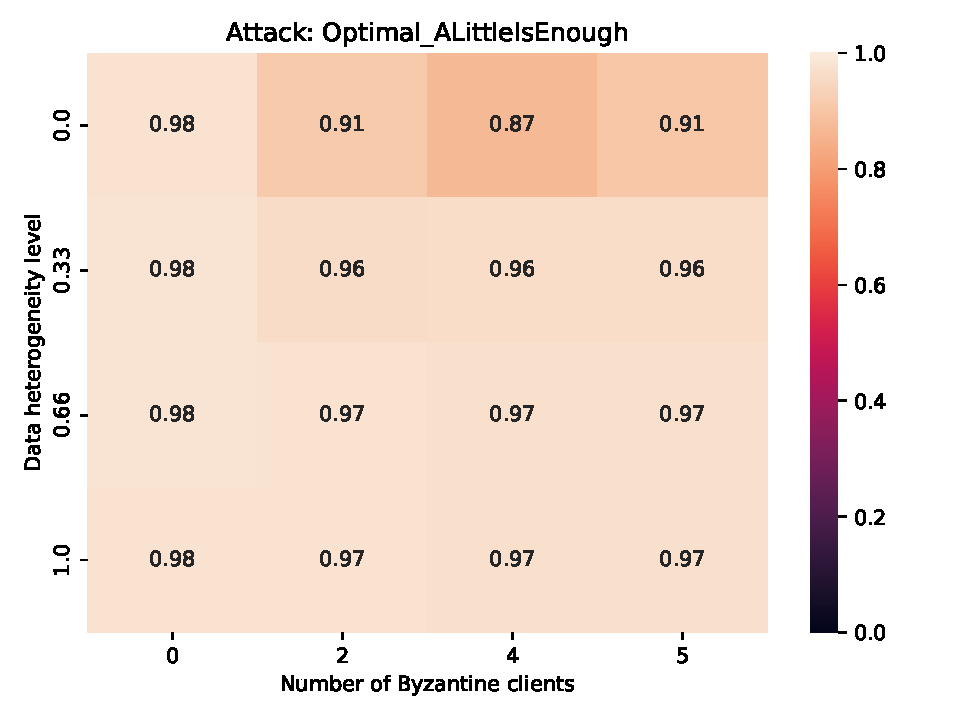
\includegraphics[width=\textwidth]{cnn_simplest_plots/test_Optimal_ALittleIsEnough_mnist_cnn_mnist_gamma_similarity_niid_NNM_ARC_CenteredClipping_nb_honest_clients_10_tolerated_f_equal_real.pdf}
        \caption{CNN (Centered Clipping)}
        \label{fig:alie_cc_cnn}
    \end{subfigure}
    \hfill
    \begin{subfigure}[b]{0.49\textwidth}
        \centering
        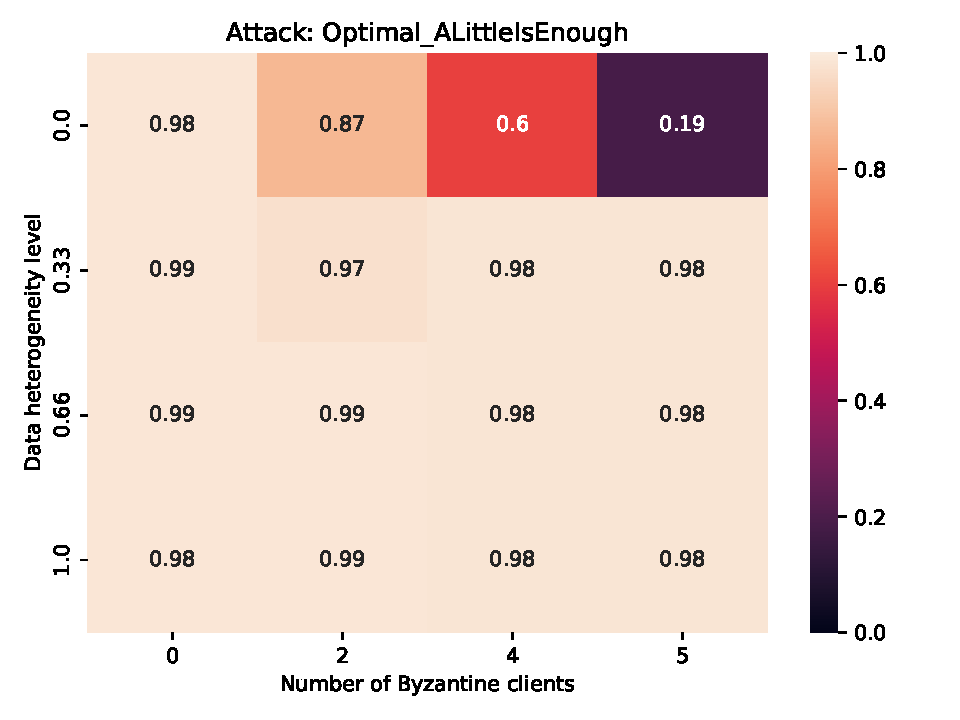
\includegraphics[width=\textwidth]{snn_simplest_plots/test_Optimal_ALittleIsEnough_mnist_cnn_mnist_snn_gamma_similarity_niid_NNM_ARC_CenteredClipping_nb_honest_clients_10_tolerated_f_equal_real.pdf}
        \caption{SNN (Centered Clipping)}
        \label{fig:alie_cc_snn}
    \end{subfigure}
    \caption{Accuracy comparison under Optimal ALIE attack using Centered Clipping.}
    \label{fig:alie_cc_comparison}
\end{figure}

\clearpage

\subsection{Geometric Median}
\begin{figure}[htbp]
    \centering
    \begin{subfigure}[b]{0.49\textwidth}
        \centering
        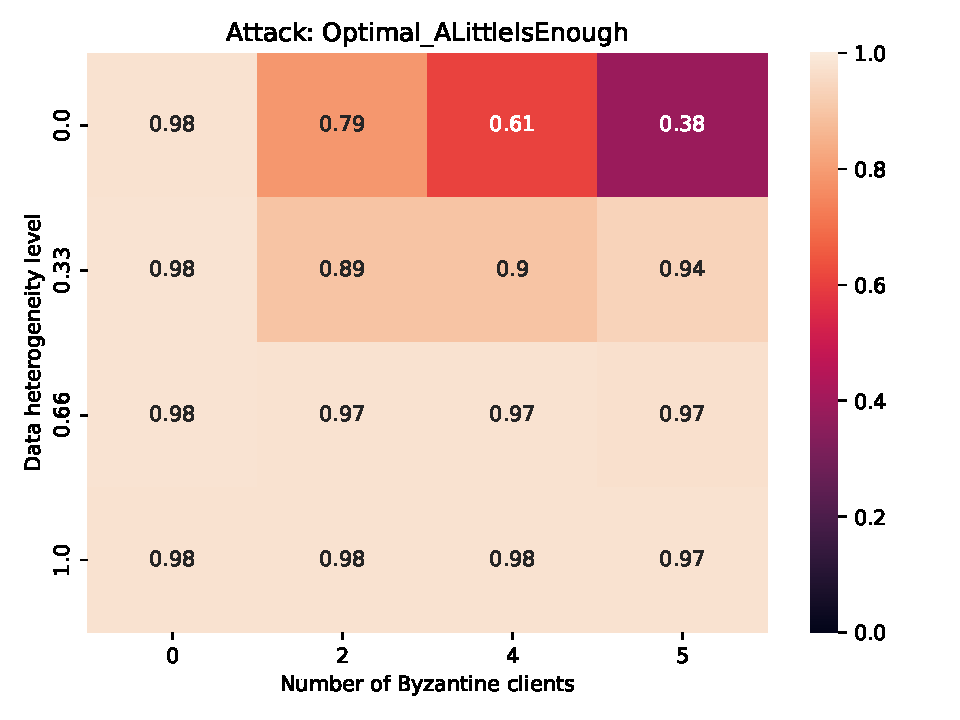
\includegraphics[width=\textwidth]{cnn_simplest_plots/test_Optimal_ALittleIsEnough_mnist_cnn_mnist_gamma_similarity_niid_NNM_ARC_GeometricMedian_nb_honest_clients_10_tolerated_f_equal_real.pdf}
        \caption{CNN (Geometric Median)}
        \label{fig:alie_gm_cnn}
    \end{subfigure}
    \hfill
    \begin{subfigure}[b]{0.49\textwidth}
        \centering
        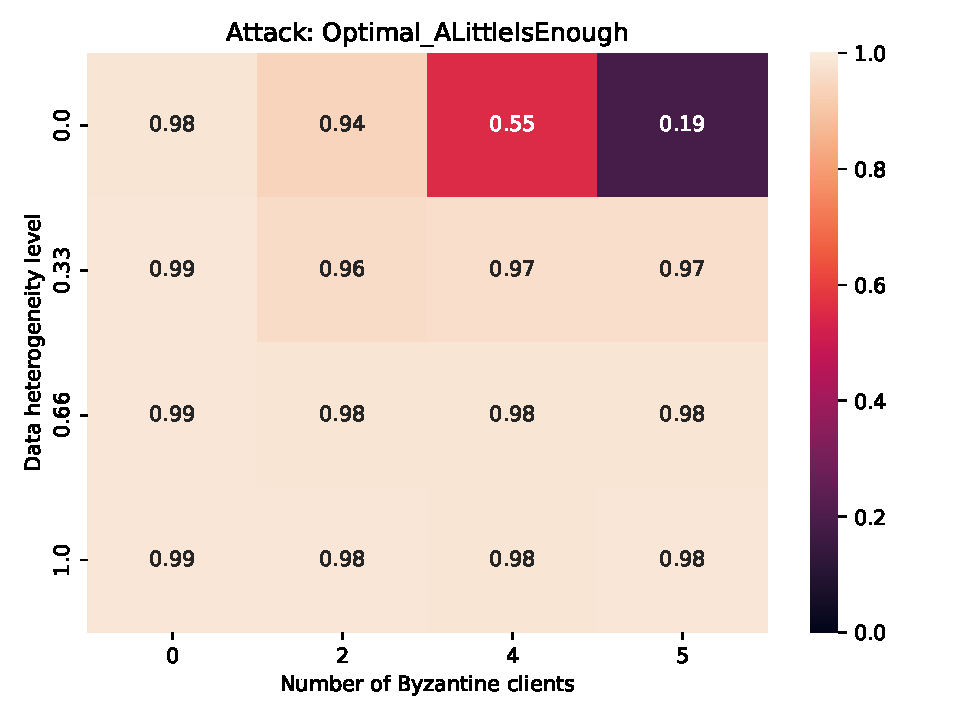
\includegraphics[width=\textwidth]{snn_simplest_plots/test_Optimal_ALittleIsEnough_mnist_cnn_mnist_snn_gamma_similarity_niid_NNM_ARC_GeometricMedian_nb_honest_clients_10_tolerated_f_equal_real.pdf}
        \caption{SNN (Geometric Median)}
        \label{fig:alie_gm_snn}
    \end{subfigure}
    \caption{Accuracy comparison under Optimal ALIE attack using Geometric Median.}
    \label{fig:alie_gm_comparison}
\end{figure}

\clearpage

\subsection{Multi-Krum}
\begin{figure}[htbp]
    \centering
    \begin{subfigure}[b]{0.49\textwidth}
        \centering
        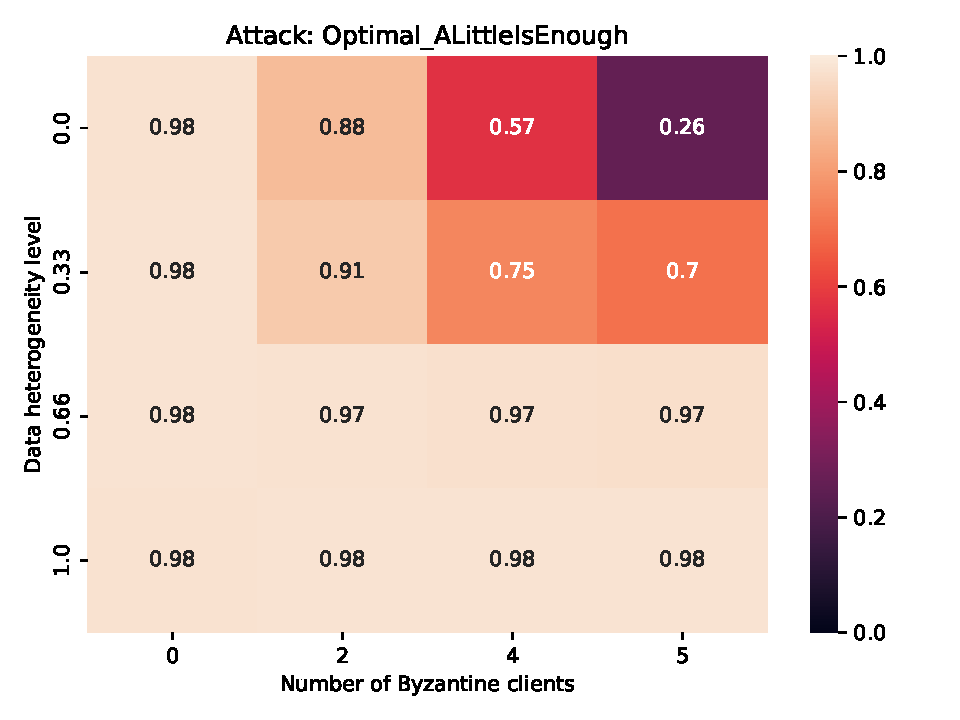
\includegraphics[width=\textwidth]{cnn_simplest_plots/test_Optimal_ALittleIsEnough_mnist_cnn_mnist_gamma_similarity_niid_NNM_ARC_MultiKrum_nb_honest_clients_10_tolerated_f_equal_real.pdf}
        \caption{CNN (Multi-Krum)}
        \label{fig:alie_mk_cnn}
    \end{subfigure}
    \hfill
    \begin{subfigure}[b]{0.49\textwidth}
        \centering
        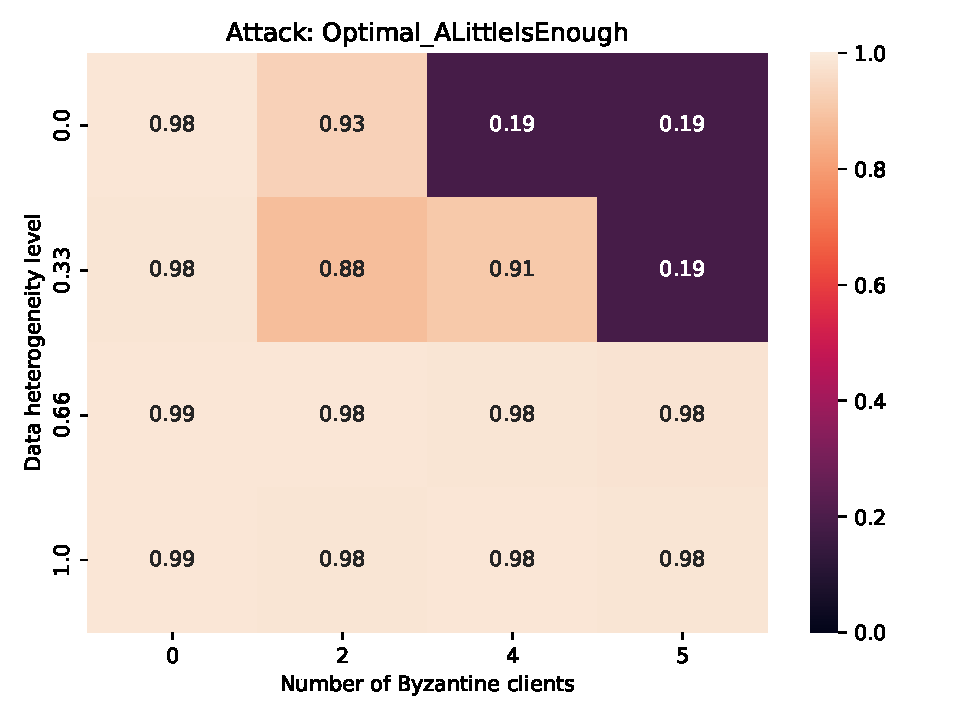
\includegraphics[width=\textwidth]{snn_simplest_plots/test_Optimal_ALittleIsEnough_mnist_cnn_mnist_snn_gamma_similarity_niid_NNM_ARC_MultiKrum_nb_honest_clients_10_tolerated_f_equal_real.pdf}
        \caption{SNN (Multi-Krum)}
        \label{fig:alie_mk_snn}
    \end{subfigure}
    \caption{Accuracy comparison under Optimal ALIE attack using Multi-Krum.}
    \label{fig:alie_mk_comparison}
\end{figure}

\clearpage

\subsection{Trimmed Mean}
\begin{figure}[htbp]
    \centering
    \begin{subfigure}[b]{0.49\textwidth}
        \centering
        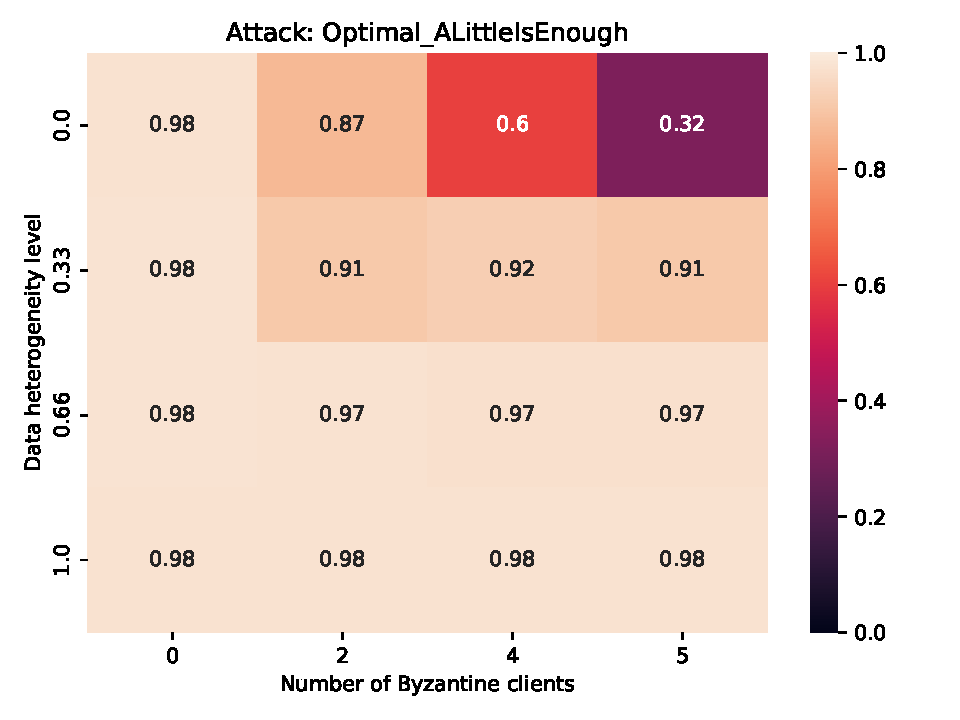
\includegraphics[width=\textwidth]{cnn_simplest_plots/test_Optimal_ALittleIsEnough_mnist_cnn_mnist_gamma_similarity_niid_NNM_ARC_TrMean_nb_honest_clients_10_tolerated_f_equal_real.pdf}
        \caption{CNN (Trimmed Mean)}
        \label{fig:alie_tm_cnn}
    \end{subfigure}
    \hfill
    \begin{subfigure}[b]{0.49\textwidth}
        \centering
        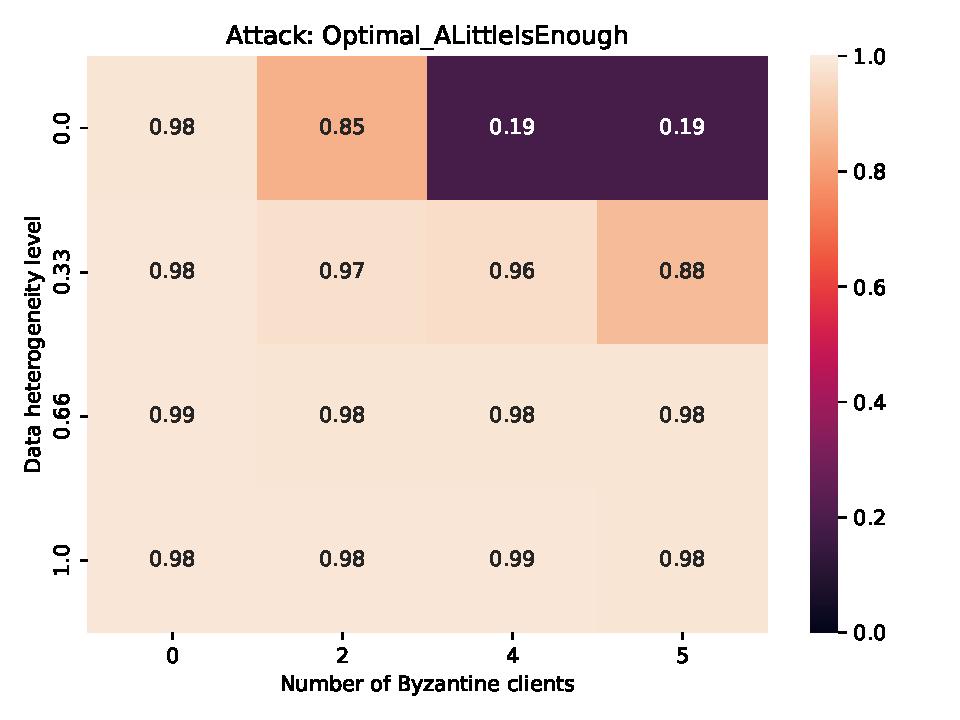
\includegraphics[width=\textwidth]{snn_simplest_plots/test_Optimal_ALittleIsEnough_mnist_cnn_mnist_snn_gamma_similarity_niid_NNM_ARC_TrMean_nb_honest_clients_10_tolerated_f_equal_real.pdf}
        \caption{SNN (Trimmed Mean)}
        \label{fig:alie_tm_snn}
    \end{subfigure}
    \caption{Accuracy comparison under Optimal ALIE attack using Trimmed Mean.}
    \label{fig:alie_tm_comparison}
\end{figure}

\clearpage

\section{Fixed Attack: Optimal Inner Product Manipulation (IPM)}
\label{sec:ipm_attack}
This section compares performance under the Optimal IPM Byzantine attack, showing both the dynamically selected best aggregator and each of the fixed aggregators.

\subsection{Best Aggregator Choice}
\begin{figure}[htbp]
    \centering
    \begin{subfigure}[b]{0.49\textwidth}
        \centering
        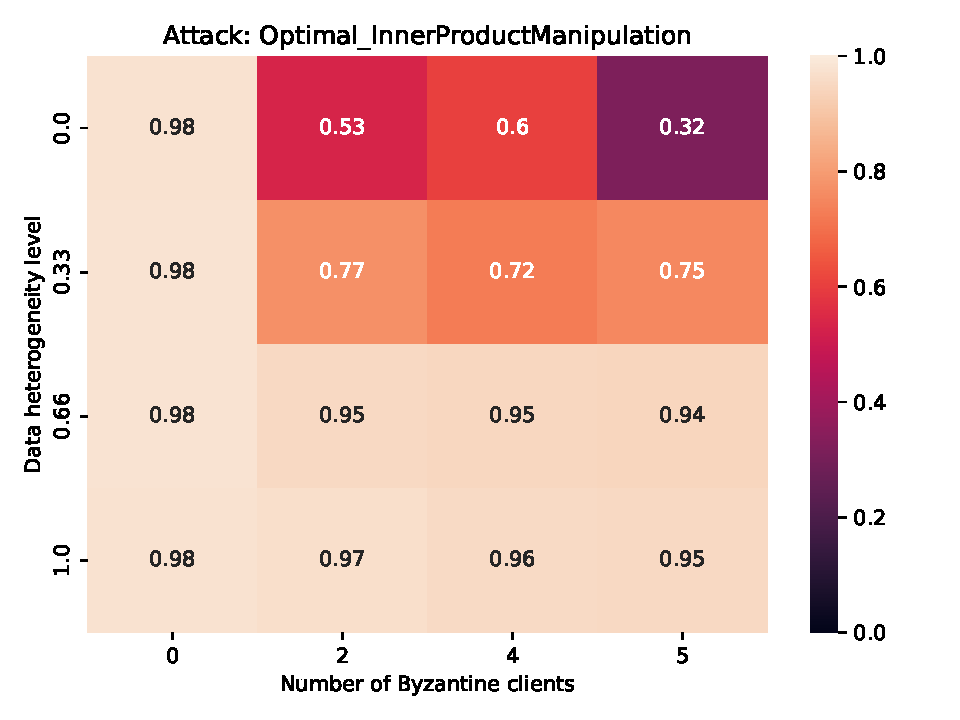
\includegraphics[width=\textwidth]{cnn_simplest_plots/best_test_Optimal_InnerProductManipulation_mnist_cnn_mnist_gamma_similarity_niid_NNM_ARC_nb_honest_clients_10_tolerated_f_equal_real.pdf}
        \caption{CNN (Best Aggregator Choice)}
        \label{fig:ipm_best_cnn}
    \end{subfigure}
    \hfill
    \begin{subfigure}[b]{0.49\textwidth}
        \centering
        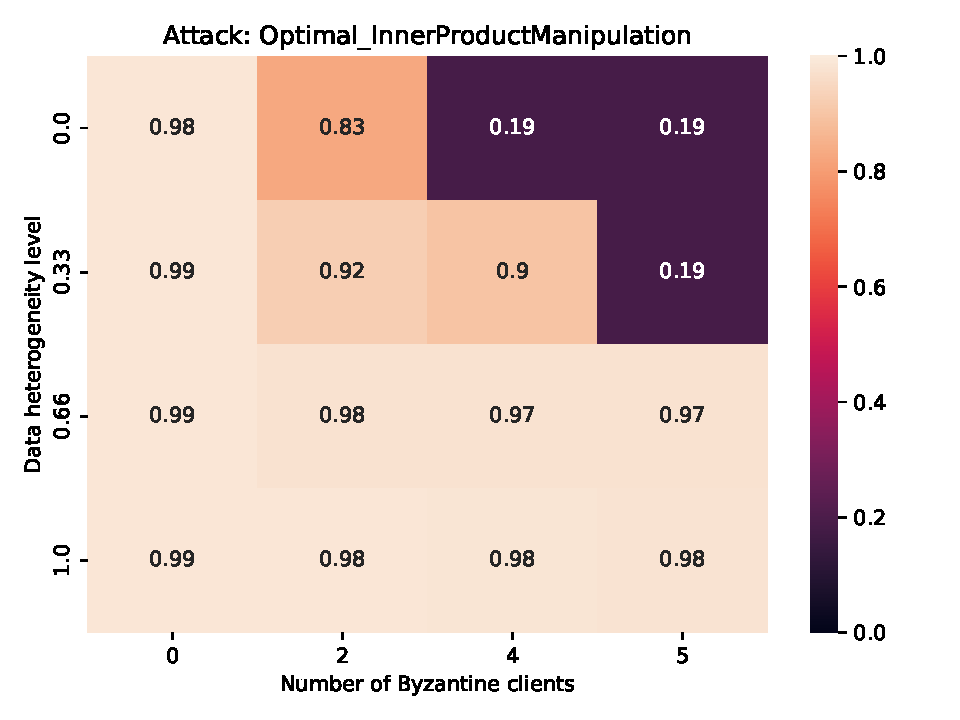
\includegraphics[width=\textwidth]{snn_simplest_plots/best_test_Optimal_InnerProductManipulation_mnist_cnn_mnist_snn_gamma_similarity_niid_NNM_ARC_nb_honest_clients_10_tolerated_f_equal_real.pdf}
        \caption{SNN (Best Aggregator Choice)}
        \label{fig:ipm_best_snn}
    \end{subfigure}
    \caption{Accuracy comparison under Optimal IPM attack using the best aggregator selection.}
    \label{fig:ipm_best_overall}
\end{figure}

\clearpage

\subsection{Centered Clipping}
\begin{figure}[htbp]
    \centering
    \begin{subfigure}[b]{0.49\textwidth}
        \centering
        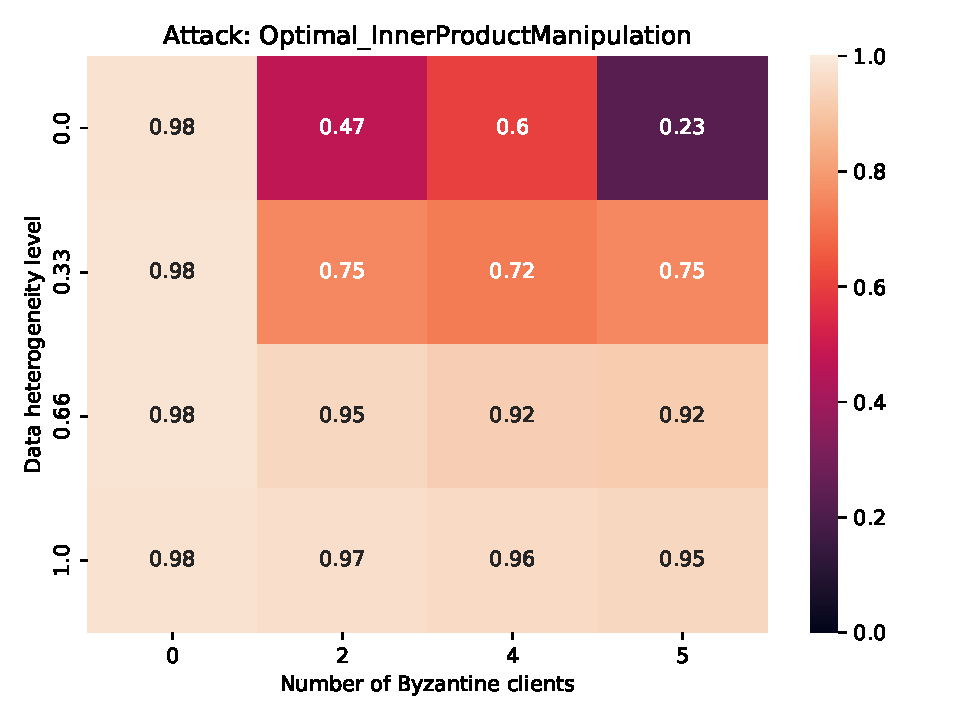
\includegraphics[width=\textwidth]{cnn_simplest_plots/test_Optimal_InnerProductManipulation_mnist_cnn_mnist_gamma_similarity_niid_NNM_ARC_CenteredClipping_nb_honest_clients_10_tolerated_f_equal_real.pdf}
        \caption{CNN (Centered Clipping)}
        \label{fig:ipm_cc_cnn}
    \end{subfigure}
    \hfill
    \begin{subfigure}[b]{0.49\textwidth}
        \centering
        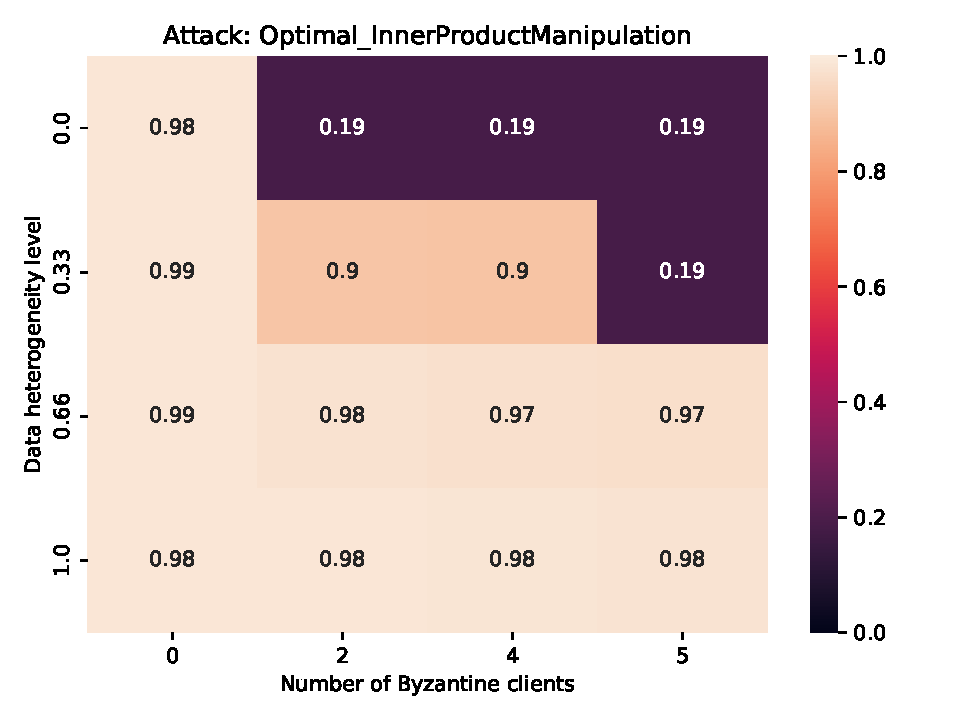
\includegraphics[width=\textwidth]{snn_simplest_plots/test_Optimal_InnerProductManipulation_mnist_cnn_mnist_snn_gamma_similarity_niid_NNM_ARC_CenteredClipping_nb_honest_clients_10_tolerated_f_equal_real.pdf}
        \caption{SNN (Centered Clipping)}
        \label{fig:ipm_cc_snn}
    \end{subfigure}
    \caption{Accuracy comparison under Optimal IPM attack using Centered Clipping.}
    \label{fig:ipm_cc_comparison}
\end{figure}

\clearpage

\subsection{Geometric Median}
\begin{figure}[htbp]
    \centering
    \begin{subfigure}[b]{0.49\textwidth}
        \centering
        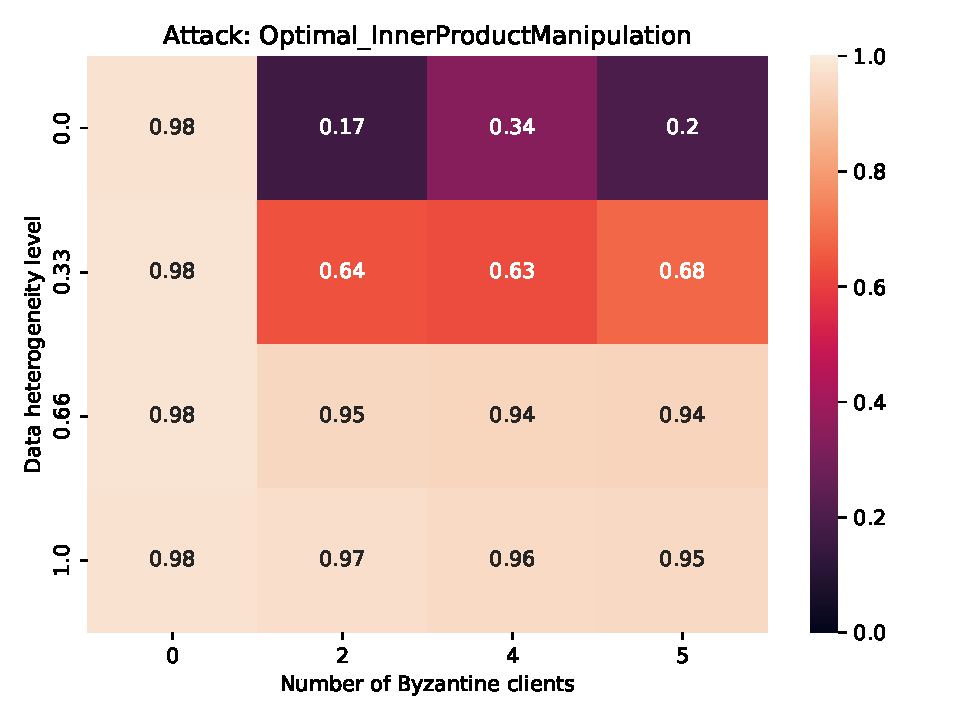
\includegraphics[width=\textwidth]{cnn_simplest_plots/test_Optimal_InnerProductManipulation_mnist_cnn_mnist_gamma_similarity_niid_NNM_ARC_GeometricMedian_nb_honest_clients_10_tolerated_f_equal_real.pdf}
        \caption{CNN (Geometric Median)}
        \label{fig:ipm_gm_cnn}
    \end{subfigure}
    \hfill
    \begin{subfigure}[b]{0.49\textwidth}
        \centering
        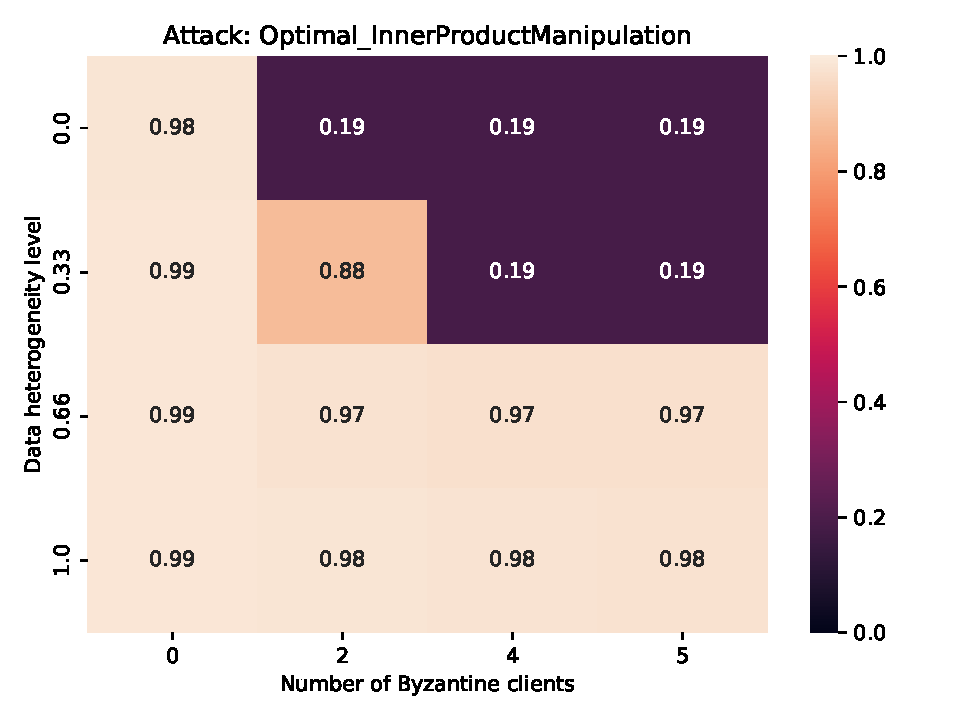
\includegraphics[width=\textwidth]{snn_simplest_plots/test_Optimal_InnerProductManipulation_mnist_cnn_mnist_snn_gamma_similarity_niid_NNM_ARC_GeometricMedian_nb_honest_clients_10_tolerated_f_equal_real.pdf}
        \caption{SNN (Geometric Median)}
        \label{fig:ipm_gm_snn}
    \end{subfigure}
    \caption{Accuracy comparison under Optimal IPM attack using Geometric Median.}
    \label{fig:ipm_gm_comparison}
\end{figure}

\clearpage

\subsection{Multi-Krum}
\begin{figure}[htbp]
    \centering
    \begin{subfigure}[b]{0.49\textwidth}
        \centering
        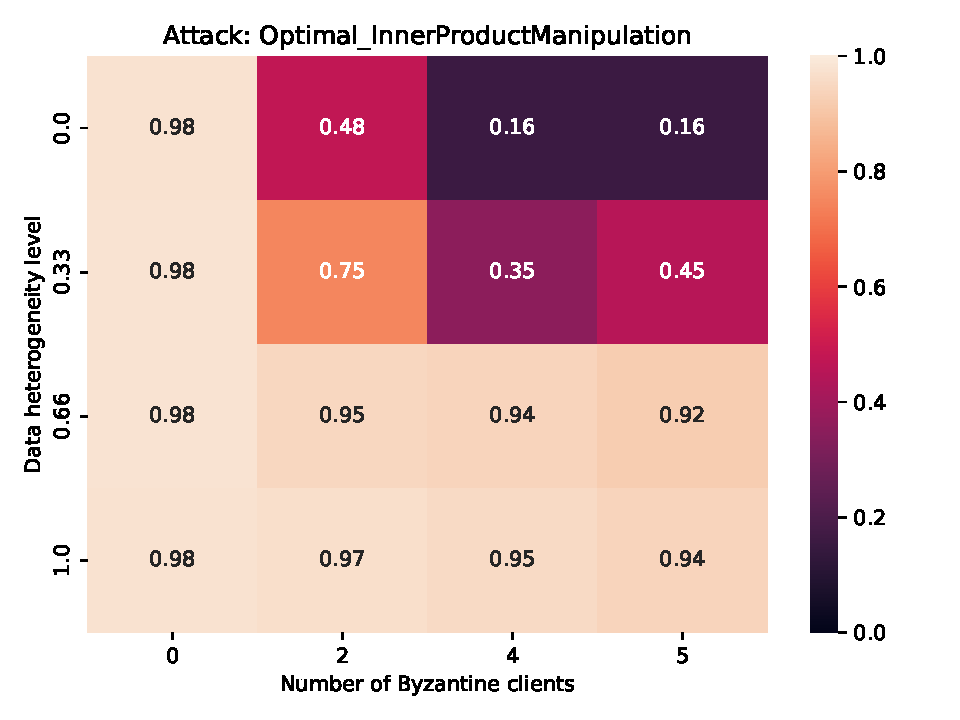
\includegraphics[width=\textwidth]{cnn_simplest_plots/test_Optimal_InnerProductManipulation_mnist_cnn_mnist_gamma_similarity_niid_NNM_ARC_MultiKrum_nb_honest_clients_10_tolerated_f_equal_real.pdf}
        \caption{CNN (Multi-Krum)}
        \label{fig:ipm_mk_cnn}
    \end{subfigure}
    \hfill
    \begin{subfigure}[b]{0.49\textwidth}
        \centering
        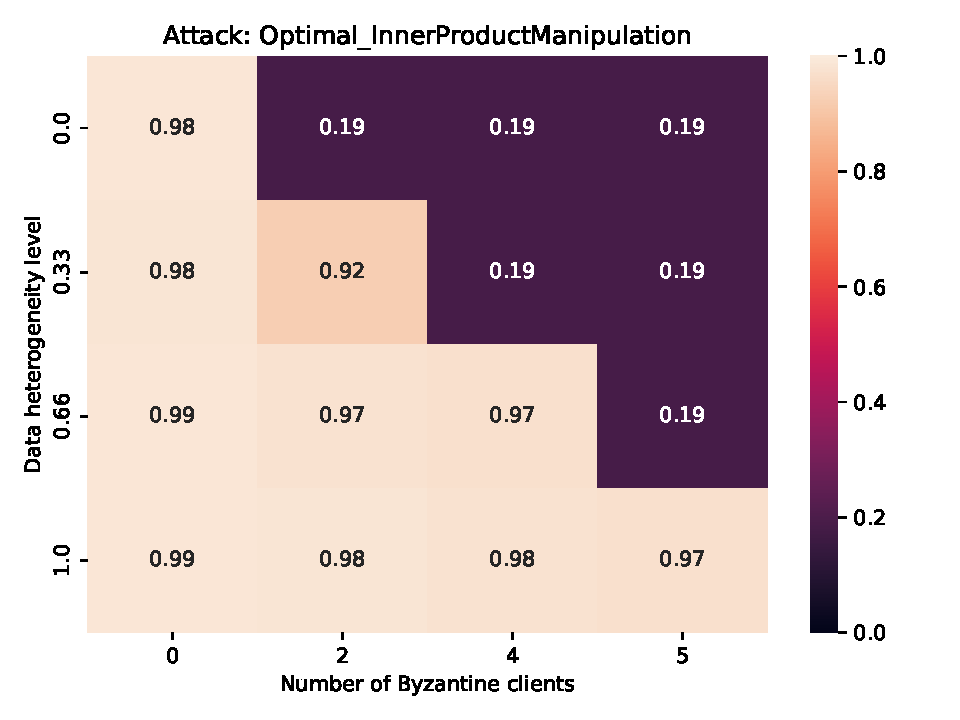
\includegraphics[width=\textwidth]{snn_simplest_plots/test_Optimal_InnerProductManipulation_mnist_cnn_mnist_snn_gamma_similarity_niid_NNM_ARC_MultiKrum_nb_honest_clients_10_tolerated_f_equal_real.pdf}
        \caption{SNN (Multi-Krum)}
        \label{fig:ipm_mk_snn}
    \end{subfigure}
    \caption{Accuracy comparison under Optimal IPM attack using Multi-Krum.}
    \label{fig:ipm_mk_comparison}
\end{figure}

\clearpage

\subsection{Trimmed Mean}
\begin{figure}[htbp]
    \centering
    \begin{subfigure}[b]{0.49\textwidth}
        \centering
        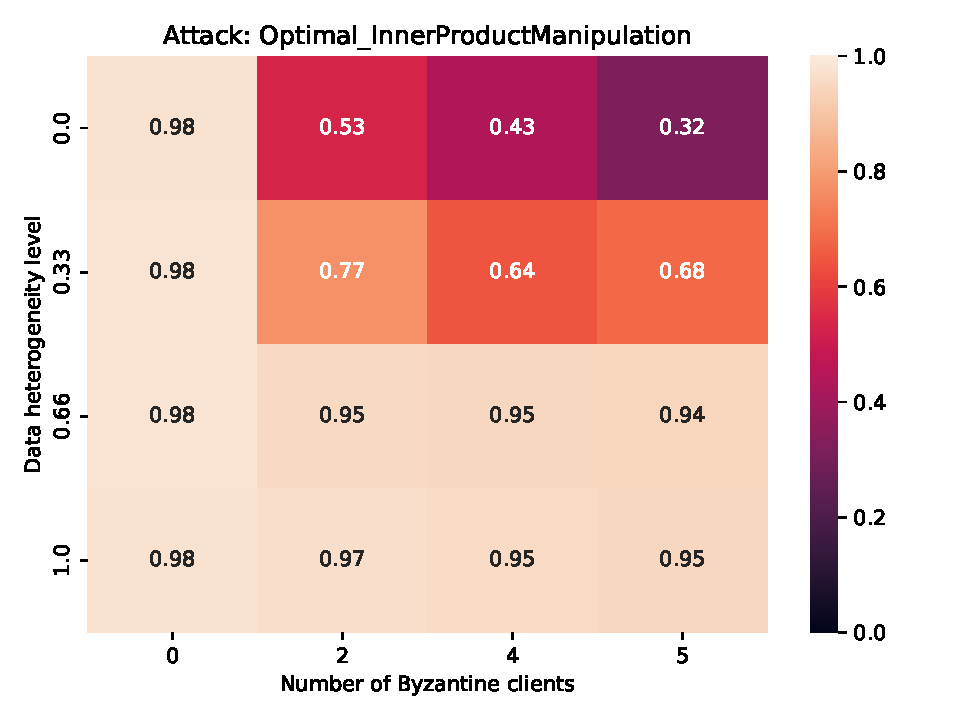
\includegraphics[width=\textwidth]{cnn_simplest_plots/test_Optimal_InnerProductManipulation_mnist_cnn_mnist_gamma_similarity_niid_NNM_ARC_TrMean_nb_honest_clients_10_tolerated_f_equal_real.pdf}
        \caption{CNN (Trimmed Mean)}
        \label{fig:ipm_tm_cnn}
    \end{subfigure}
    \hfill
    \begin{subfigure}[b]{0.49\textwidth}
        \centering
        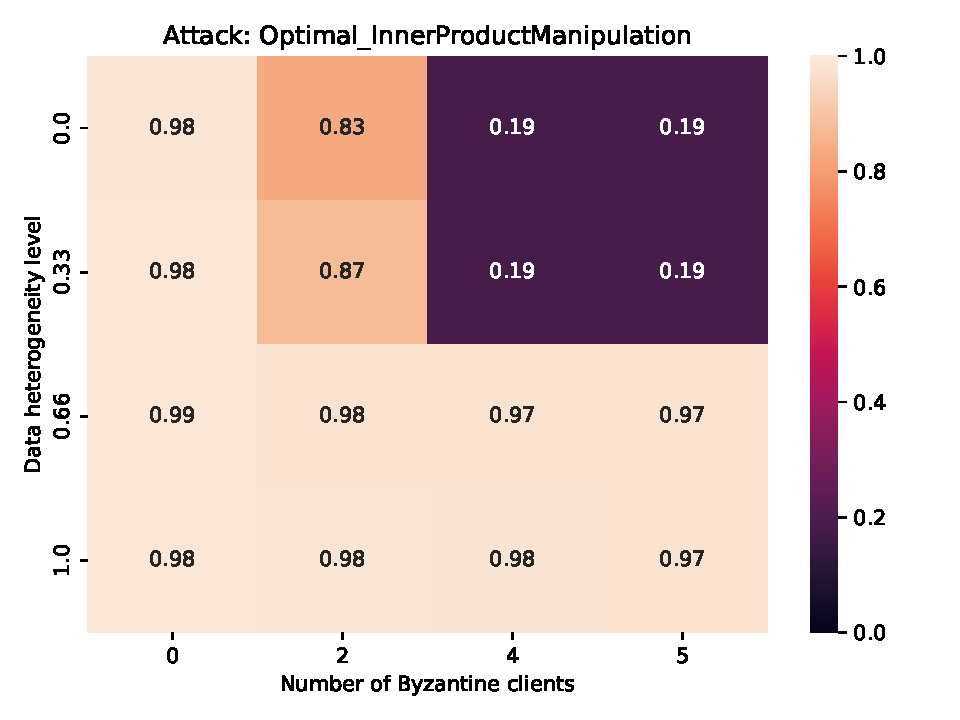
\includegraphics[width=\textwidth]{snn_simplest_plots/test_Optimal_InnerProductManipulation_mnist_cnn_mnist_snn_gamma_similarity_niid_NNM_ARC_TrMean_nb_honest_clients_10_tolerated_f_equal_real.pdf}
        \caption{SNN (Trimmed Mean)}
        \label{fig:ipm_tm_snn}
    \end{subfigure}
    \caption{Accuracy comparison under Optimal IPM attack using Trimmed Mean.}
    \label{fig:ipm_tm_comparison}
\end{figure}

\clearpage

\section{Fixed Attack: Sign Flipping}
\label{sec:sign_flipping_attack}
This section compares performance under the Sign Flipping Byzantine attack, showing both the dynamically selected best aggregator and each of the fixed aggregators.

\subsection{Best Aggregator Choice}
\begin{figure}[htbp]
    \centering
    \begin{subfigure}[b]{0.49\textwidth}
        \centering
        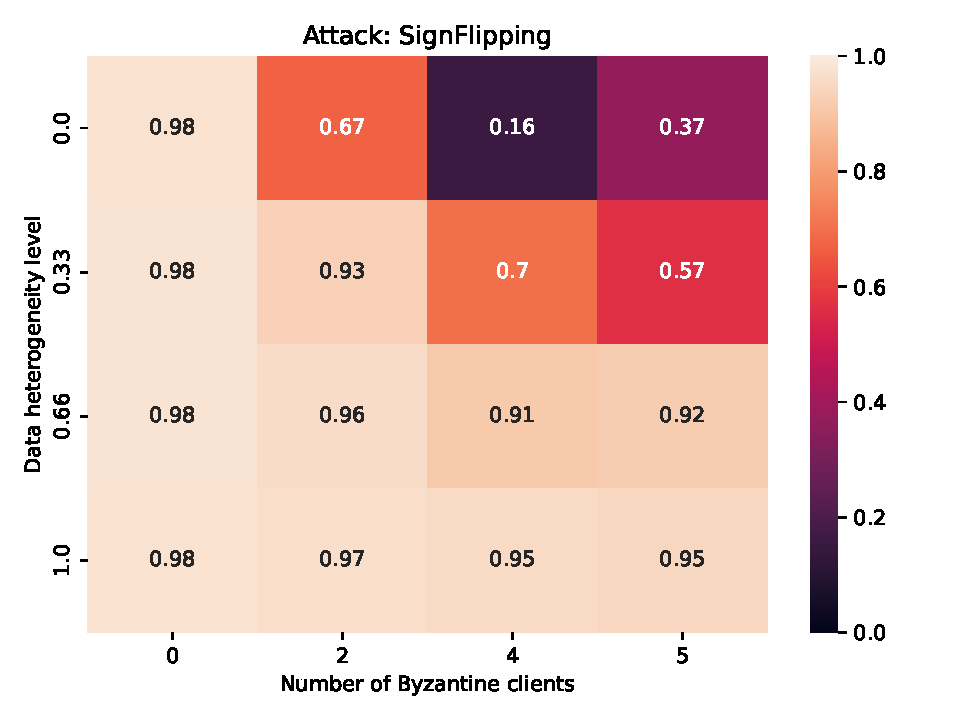
\includegraphics[width=\textwidth]{cnn_simplest_plots/best_test_SignFlipping_mnist_cnn_mnist_gamma_similarity_niid_NNM_ARC_nb_honest_clients_10_tolerated_f_equal_real.pdf}
        \caption{CNN (Best Aggregator Choice)}
        \label{fig:sf_best_cnn}
    \end{subfigure}
    \hfill
    \begin{subfigure}[b]{0.49\textwidth}
        \centering
        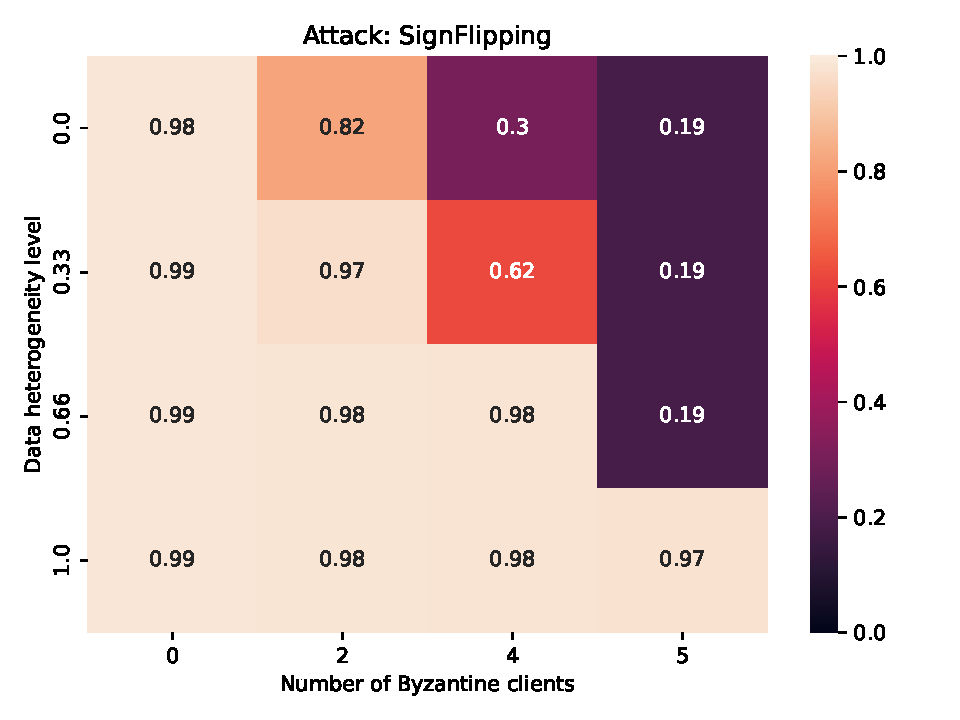
\includegraphics[width=\textwidth]{snn_simplest_plots/best_test_SignFlipping_mnist_cnn_mnist_snn_gamma_similarity_niid_NNM_ARC_nb_honest_clients_10_tolerated_f_equal_real.pdf}
        \caption{SNN (Best Aggregator Choice)}
        \label{fig:sf_best_snn}
    \end{subfigure}
    \caption{Accuracy comparison under Sign Flipping attack using the best aggregator selection.}
    \label{fig:sf_best_overall}
\end{figure}

\clearpage

\subsection{Centered Clipping}
\begin{figure}[htbp]
    \centering
    \begin{subfigure}[b]{0.49\textwidth}
        \centering
        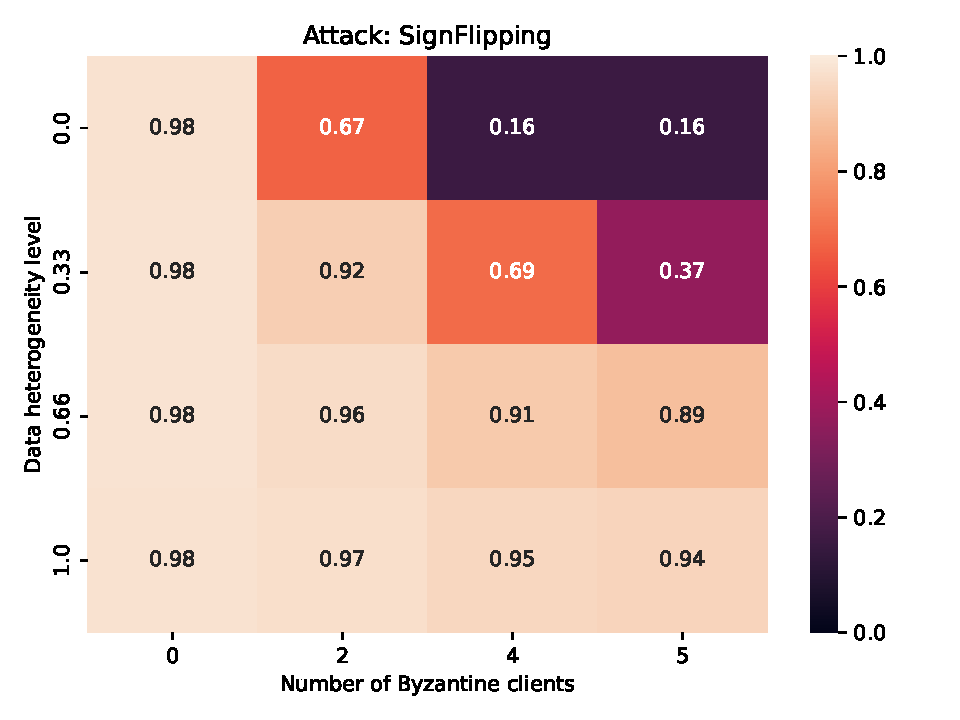
\includegraphics[width=\textwidth]{cnn_simplest_plots/test_SignFlipping_mnist_cnn_mnist_gamma_similarity_niid_NNM_ARC_CenteredClipping_nb_honest_clients_10_tolerated_f_equal_real.pdf}
        \caption{CNN (Centered Clipping)}
        \label{fig:sf_cc_cnn}
    \end{subfigure}
    \hfill
    \begin{subfigure}[b]{0.49\textwidth}
        \centering
        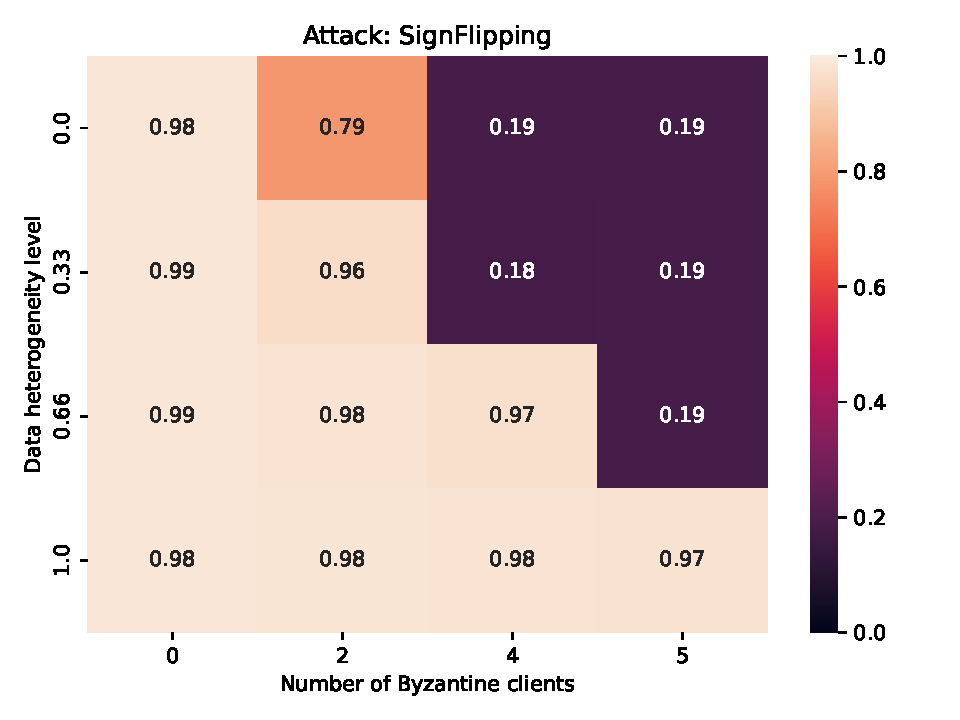
\includegraphics[width=\textwidth]{snn_simplest_plots/test_SignFlipping_mnist_cnn_mnist_snn_gamma_similarity_niid_NNM_ARC_CenteredClipping_nb_honest_clients_10_tolerated_f_equal_real.pdf}
        \caption{SNN (Centered Clipping)}
        \label{fig:sf_cc_snn}
    \end{subfigure}
    \caption{Accuracy comparison under Sign Flipping attack using Centered Clipping.}
    \label{fig:sf_cc_comparison}
\end{figure}

\clearpage

\subsection{Geometric Median}
\begin{figure}[htbp]
    \centering
    \begin{subfigure}[b]{0.49\textwidth}
        \centering
        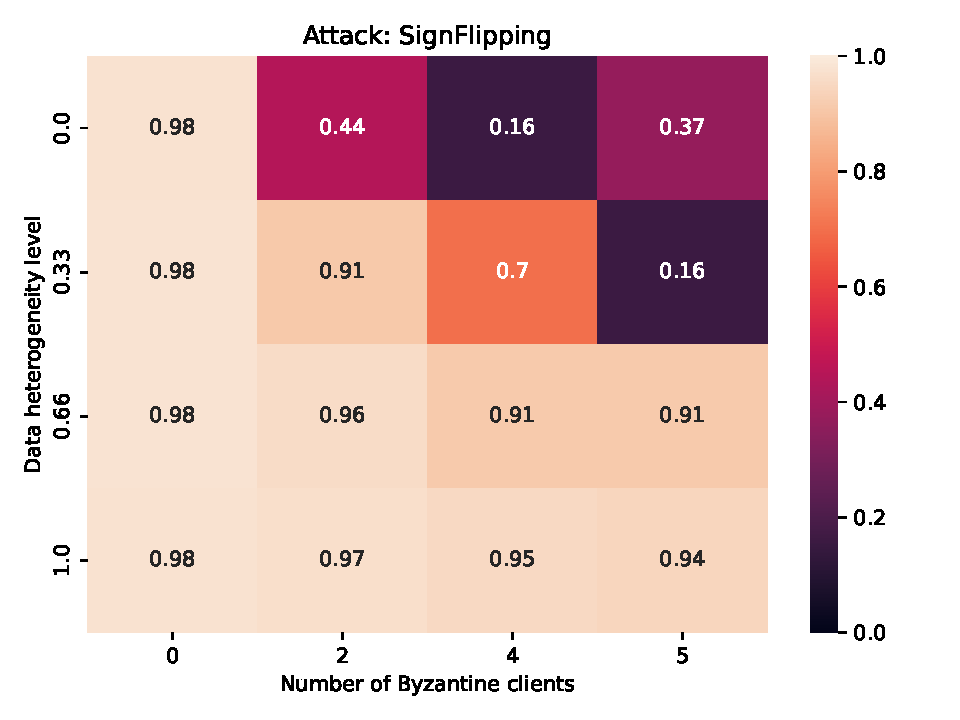
\includegraphics[width=\textwidth]{cnn_simplest_plots/test_SignFlipping_mnist_cnn_mnist_gamma_similarity_niid_NNM_ARC_GeometricMedian_nb_honest_clients_10_tolerated_f_equal_real.pdf}
        \caption{CNN (Geometric Median)}
        \label{fig:sf_gm_cnn}
    \end{subfigure}
    \hfill
    \begin{subfigure}[b]{0.49\textwidth}
        \centering
        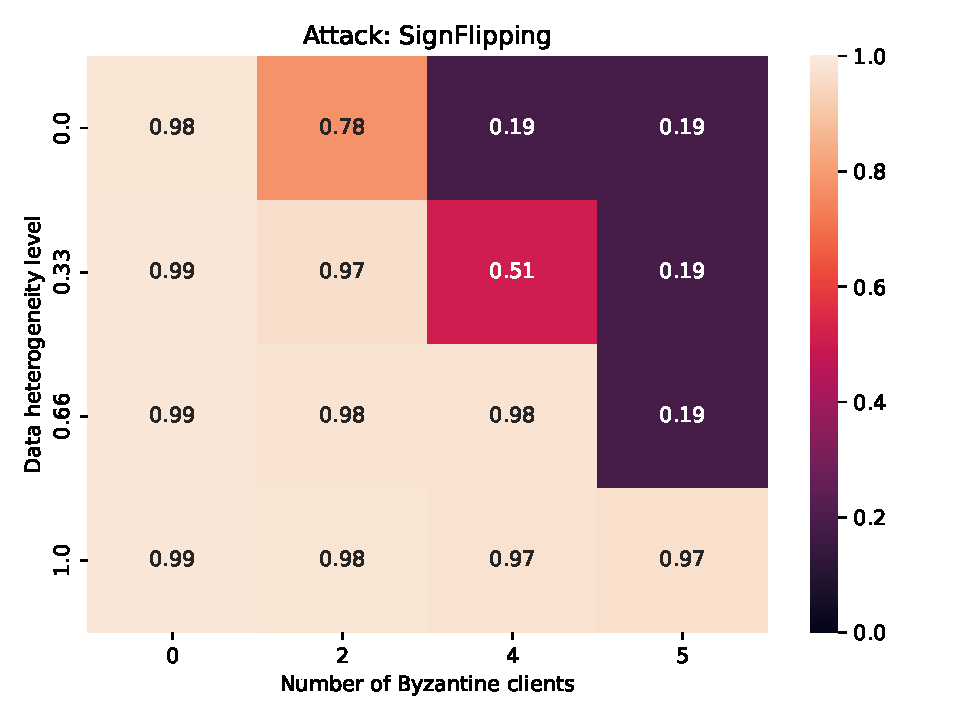
\includegraphics[width=\textwidth]{snn_simplest_plots/test_SignFlipping_mnist_cnn_mnist_snn_gamma_similarity_niid_NNM_ARC_GeometricMedian_nb_honest_clients_10_tolerated_f_equal_real.pdf}
        \caption{SNN (Geometric Median)}
        \label{fig:sf_gm_snn}
    \end{subfigure}
    \caption{Accuracy comparison under Sign Flipping attack using Geometric Median.}
    \label{fig:sf_gm_comparison}
\end{figure}

\clearpage

\subsection{Multi-Krum}
\begin{figure}[htbp]
    \centering
    \begin{subfigure}[b]{0.49\textwidth}
        \centering
        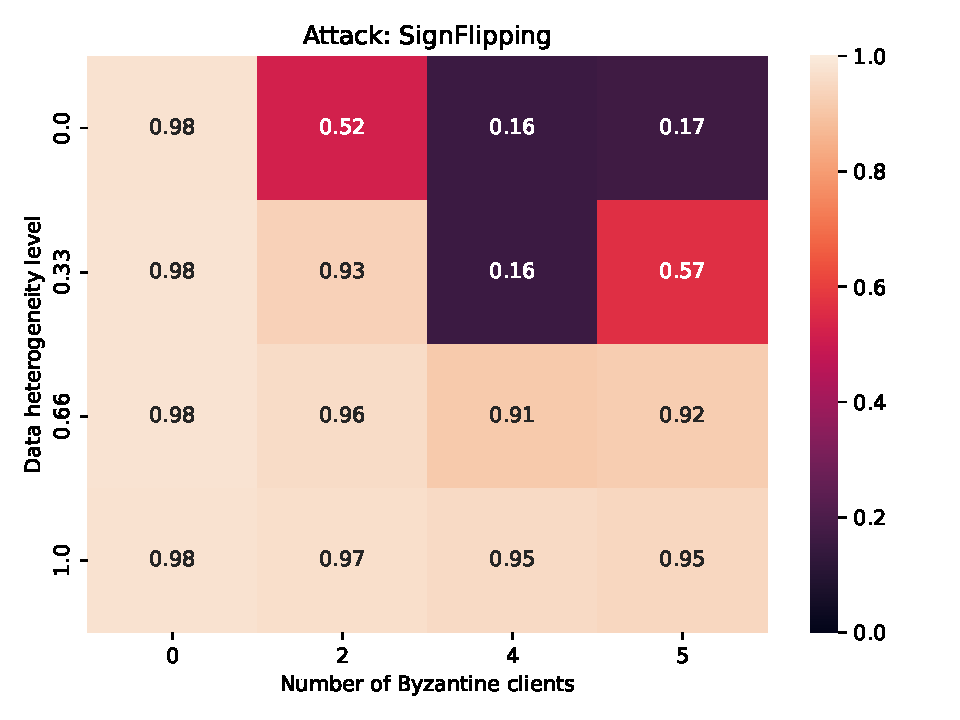
\includegraphics[width=\textwidth]{cnn_simplest_plots/test_SignFlipping_mnist_cnn_mnist_gamma_similarity_niid_NNM_ARC_MultiKrum_nb_honest_clients_10_tolerated_f_equal_real.pdf}
        \caption{CNN (Multi-Krum)}
        \label{fig:sf_mk_cnn}
    \end{subfigure}
    \hfill
    \begin{subfigure}[b]{0.49\textwidth}
        \centering
        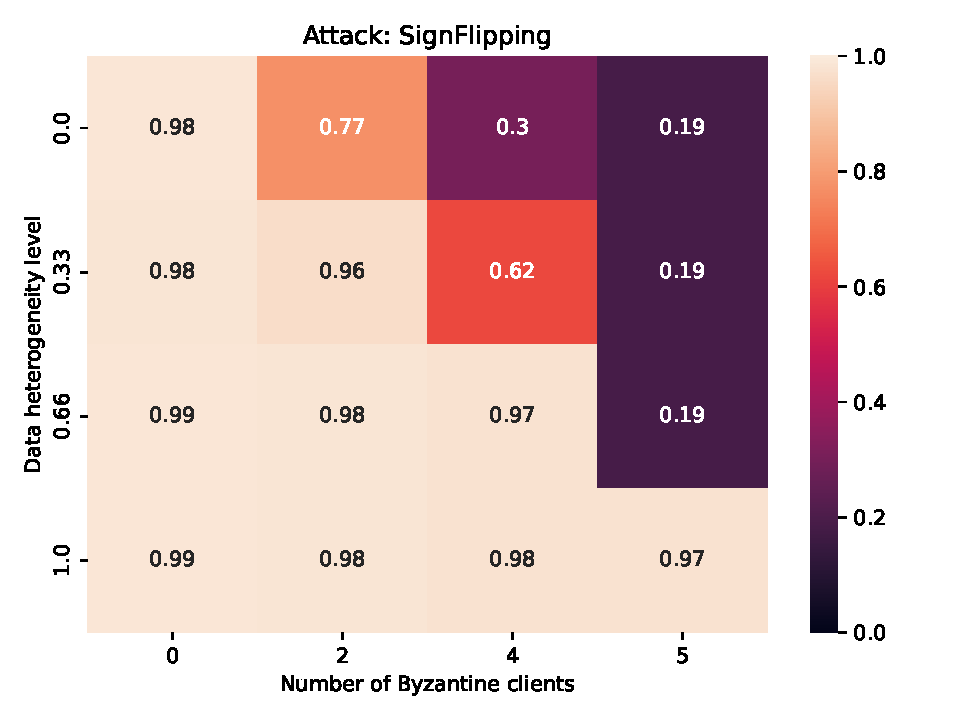
\includegraphics[width=\textwidth]{snn_simplest_plots/test_SignFlipping_mnist_cnn_mnist_snn_gamma_similarity_niid_NNM_ARC_MultiKrum_nb_honest_clients_10_tolerated_f_equal_real.pdf}
        \caption{SNN (Multi-Krum)}
        \label{fig:sf_mk_snn}
    \end{subfigure}
    \caption{Accuracy comparison under Sign Flipping attack using Multi-Krum.}
    \label{fig:sf_mk_comparison}
\end{figure}

\clearpage

\subsection{Trimmed Mean}
\begin{figure}[htbp]
    \centering
    \begin{subfigure}[b]{0.49\textwidth}
        \centering
        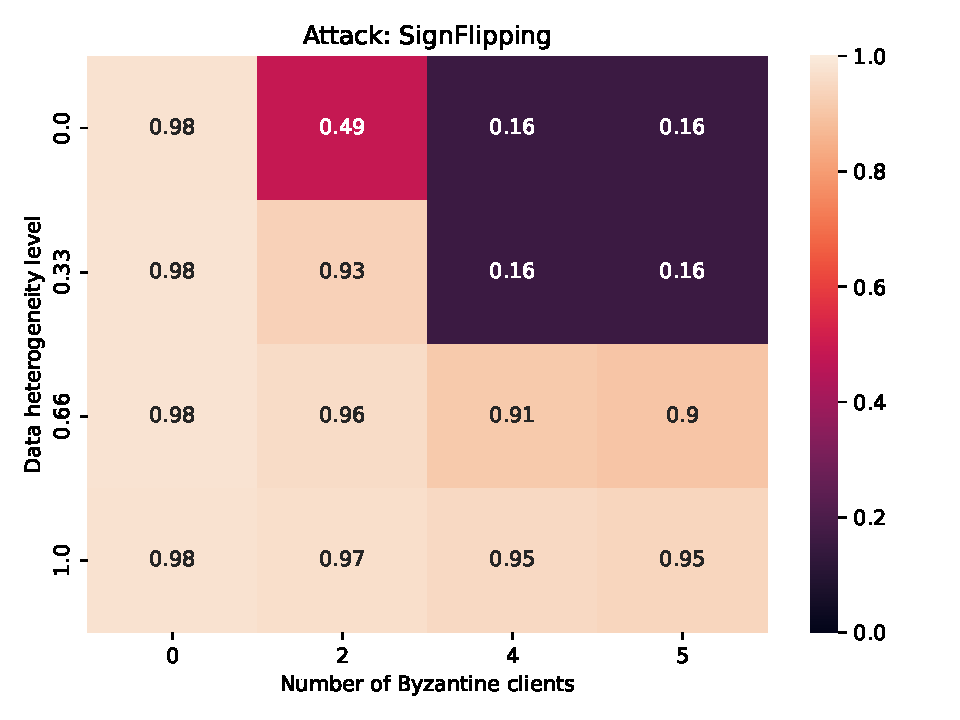
\includegraphics[width=\textwidth]{cnn_simplest_plots/test_SignFlipping_mnist_cnn_mnist_gamma_similarity_niid_NNM_ARC_TrMean_nb_honest_clients_10_tolerated_f_equal_real.pdf}
        \caption{CNN (Trimmed Mean)}
        \label{fig:sf_tm_cnn}
    \end{subfigure}
    \hfill
    \begin{subfigure}[b]{0.49\textwidth}
        \centering
        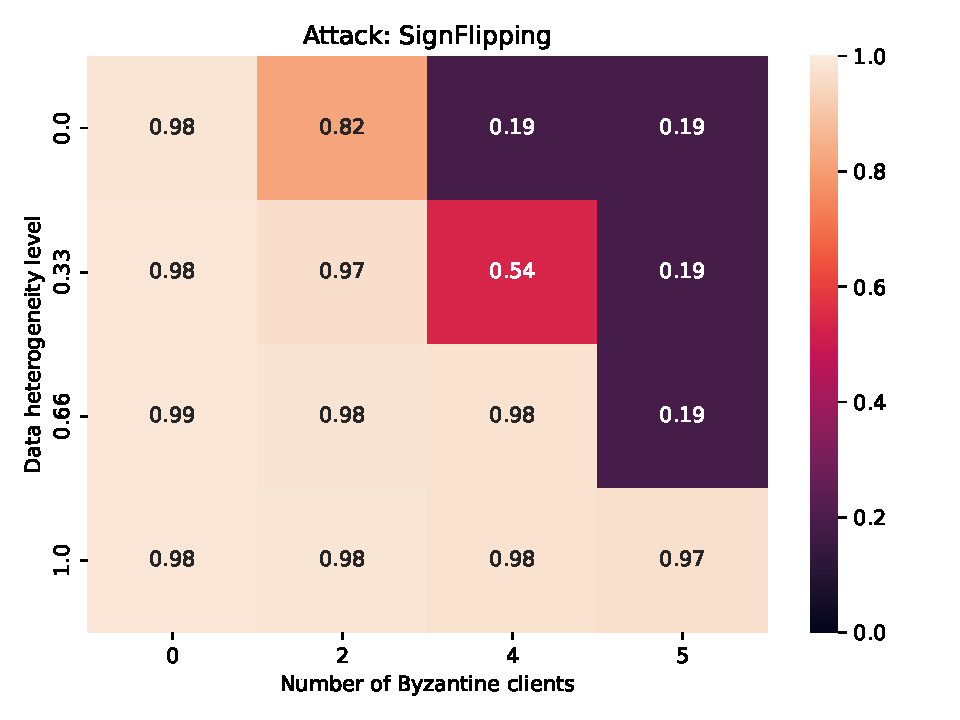
\includegraphics[width=\textwidth]{snn_simplest_plots/test_SignFlipping_mnist_cnn_mnist_snn_gamma_similarity_niid_NNM_ARC_TrMean_nb_honest_clients_10_tolerated_f_equal_real.pdf}
        \caption{SNN (Trimmed Mean)}
        \label{fig:sf_tm_snn}
    \end{subfigure}
    \caption{Accuracy comparison under Sign Flipping attack using Trimmed Mean.}
    \label{fig:sf_tm_comparison}
\end{figure}

\end{document}
